\documentclass[sigconf,review,anonymous]{acmart}

\AtBeginDocument{%
  \providecommand\BibTeX{{%
    Bib\TeX}}}

%%
%% Rights management information.
%% Update these when you receive your rights confirmation email.
%%
%\setcopyright{acmlicensed}
%\copyrightyear{2026}
%\acmYear{2026}
%\acmDOI{XXXXXXX.XXXXXXX}
%\acmConference[ASE '26]{The 41st IEEE/ACM International Conference on Automated Software Engineering}{2026}{Sacramento, California, USA}
%\acmISBN{978-1-4503-XXXX-X/2026/XX}

%%
%% Packages
%%
\usepackage{booktabs}
\usepackage{microtype}
\usepackage{xspace}
\usepackage{cleveref}
\usepackage{listings}
\usepackage{amsmath}
\usepackage{graphicx}
\usepackage{multirow}
\usepackage{xcolor}

%%
%% Macros
%%
\newcommand{\etal}{et~al\mbox{.}\xspace}
\newcommand{\ie}{i.e\mbox{.}\xspace}
\newcommand{\eg}{e.g\mbox{.}\xspace}
\newcommand{\aka}{a.k.a\mbox{.}\xspace}
\newcommand{\Triton}{\textsc{Triton}\xspace}
\newcommand{\TileLang}{\textsc{TileLang}\xspace}

\begin{document}

\title{An Empirical Study of {GPU} Kernel Performance Gaps in Modern Domain-Specific Languages}

\author{Anonymous Author(s)}
\affiliation{%
  \institution{Anonymous Institution}
  \country{}}

\begin{abstract}
  Modern GPU domain-specific languages (DSLs), such as Triton and TileLang, are increasingly used to implement specialized deep-learning kernels and as target languages for automated kernel-generation systems. Existing DSL-kernel evaluations commonly establish correctness through reference-based numerical validation. While this criterion is necessary, it does not characterize replacement quality, since a functionally valid kernel may still fall far below the latency and throughput of the optimized library operator it is intended to replace. 

We study this correctness–performance gap as an evaluation problem for GPU DSL kernels. Using 22 Triton and TileLang kernels from five operator categories on NVIDIA A100 and GH200 GPUs, we ask whether current correctness-based evaluation identifies kernels that are unsuitable as library replacements, why such failures occur, and how they can be detected without exhaustive benchmark coverage. The study yields three results. {First}, correctness-based evaluation can admit severe slowdowns: an idiomatic TileLang LayerNorm kernel passes KernelBench’s correctness check while running more than 300× slower than the PyTorch baseline. {Second}, the causes differ by kernel family. TileLang normalization and reduction slowdowns are mainly repairable authoring defects, such as sequential reductions and unnecessary dtype conversions, whereas convolution and large GEMM retain residual gaps after optimization due to code generation, autotuning coverage, and vendor-library algorithm selection. {Third}, library-relative efficiency and roofline utilization provide complementary screening criteria for identifying functionally valid but inefficient DSL kernels.
\end{abstract}

%%
%% CCS Concepts: generate at https://dl.acm.org/ccs/ccs.cfm
%%
%\begin{CCSXML}
%<ccs2012>
%   <concept>
%       <concept_id>10010520.10010521.10010537.10010540</concept_id>
%       <concept_desc>Computer systems organization~Parallel architectures</concept_desc>
%       <concept_significance>500</concept_significance>
%   </concept>
%   <concept>
%       <concept_id>10011007.10011006.10011008.10011009.10011021</concept_id>
%       <concept_desc>Software and its engineering~Domain specific languages</concept_desc>
%       <concept_significance>500</concept_significance>
%   </concept>
%   <concept>
%       <concept_id>10011007.10011074.10011099.10011692</concept_id>
%       <concept_desc>Software and its engineering~Empirical software validation</concept_desc>
%       <concept_significance>300</concept_significance>
%   </concept>
%</ccs2012>
%\end{CCSXML}
%\ccsdesc[500]{Computer systems organization~Parallel architectures}
%\ccsdesc[500]{Software and its engineering~Domain specific languages}
%\ccsdesc[300]{Software and its engineering~Empirical software validation}

\keywords{GPU kernels, domain-specific languages, Triton, TileLang, cuBLAS, cuDNN,
          empirical study, performance analysis, convolution}

\maketitle

%%% ------------------------------------------------------------------
\section{Introduction}
\label{sec:introduction}
% Introduction — pivoted framing (the DSL kernel *evaluation* problem).
% Canonical: ../PIVOT_FRAMING.md. Pre-pivot gap-study drafts are in git history.
% TODO(revision): add references.bib entries for the \cite{kernelbench} key (KernelBench,
% Ouyang et al., Stanford ScalingIntelligence) and, if used, an LLM-kernel-generation
% reward-hacking example. \cite{kernelbench} is currently undefined (non-fatal build warning).

Deep learning systems are now widely deployed, and their efficiency depends heavily on a small number of GPU kernels that dominate execution time~\cite{acceleration_survey, optimization_survey}.
Frameworks have historically delegated these kernels to vendor libraries such as cuBLAS and cuDNN~\cite{cublas2024, chetlur2014cudnn}, but modern architectures increasingly require fused operators, specialized kernels, and model-specific computations that fall outside the fixed functionality those libraries expose~\cite{kernelfusion}.
Achieving high performance therefore now depends on the ability to generate efficient \emph{custom} kernels, and domain-specific languages (DSLs) such as Triton~\cite{openai2021triton} and TileLang~\cite{wang2025tilelang} have become the standard way to write them: they express kernels at the tile level while delegating memory movement, scheduling, and code generation to a compiler.
Their reach extends well beyond hand-written code---Triton is the lowering target for \texttt{torch.compile}~\cite{li2023torchcompile}, and DSLs are increasingly the output of LLM-based kernel generators~\cite{kernelbench}---so the efficiency of DSL-generated kernels is now a first-order concern.

The difficulty is that a developer, or an automated generator, who produces a \emph{functionally correct} DSL kernel has no reliable way to tell whether it is \emph{performant}.
A correct kernel may be competitive with the vendor library, or it may be orders of magnitude slower, and nothing in the source makes the difference visible.
When a DSL-generated kernel is correct yet much slower than the corresponding library routine, the developer must determine whether the loss arises from the algorithm, the schedule, or the compiler---and current toolchains offer little diagnostic support for that distinction~\cite{gpuenergy}.
This makes performance deficits hard to predict and hard to correct, which is a software-engineering problem as much as a compiler one: a high-level kernel language is useful in practice only if its performance behavior is something developers can evaluate and reason about.

The benchmarks practitioners actually rely on do not close this gap.
The prevailing benchmarks for DSL and LLM-generated kernels---KernelBench~\cite{kernelbench} and TritonBench~\cite{li2025tritonbench}---gate on \emph{correctness}, reporting performance as an outcome rather than enforcing it as an acceptance criterion.
As a result they admit performance-poor kernels: in our measurements a naive but idiomatic TileLang kernel passes the KernelBench-style correctness gate while running more than $300\times$ slower than PyTorch, and the gate's one reward-hacking guard never fires because it only flags suspiciously \emph{fast} kernels.
These benchmarks also cover a narrow slice of the space---often a single DSL, data type, shape, and GPU per task---so a kernel that passes tells a developer little about whether it is well written.
And the obvious remedy, a benchmark comprehensive enough to span every operator, data type, shape, and architecture, is combinatorially infeasible to build and maintain.

This paper studies that evaluation problem directly.
We ask three questions: (RQ1) whether existing benchmarks can distinguish well-written DSL kernels from performance-poor ones, and where they fall short; (RQ2) for kernels that pass such benchmarks, how large and structured the hidden performance gap to vendor libraries actually is, and what causes it; and (RQ3) how to guide DSL kernel development when a comprehensive benchmark is infeasible.
We evaluate Triton and TileLang against PyTorch with cuBLAS/cuDNN on 22 kernels spanning five operator classes---GEMM, attention, convolution, normalization, and element-wise/reduction---with hardware-counter profiling via Nsight Compute.
Primary measurements span two datacenter architectures---the NVIDIA A100-SXM4-40GB (Ampere) and the NVIDIA GH200 (Grace Hopper).

Our findings are threefold.
First, the evaluation gap is real and large: naive-but-correct kernels pass the gate while running hundreds of times slower---the shipped TileLang LayerNorm is $323\times$ slower under locked clocks---and the dominant benchmarks neither gate on performance nor cover enough of the space to catch it.
Second, the hidden gap is highly structured: most is an \emph{authoring} artifact that a single reduction-primitive change (\texttt{T.serial}$\rightarrow$\texttt{T.reduce} with native-dtype I/O) repairs to library parity or better, while a residual convolution gap is structural (cuDNN's implicit-GEMM maturity; absent Winograd contributes only $\approx$2--3\%); we separate causes by \emph{where the fix belongs}---user-space authoring, code generation, and library maturity.
Third, absent a comprehensive benchmark, lightweight heuristics suffice: a library-comparability check anchored by a baseline-independent roofline fraction cleanly separates well-written kernels from poor ones, and a small set of recurring optimization patterns guides the fixes.

\smallskip\noindent\textbf{Contributions.}
\begin{itemize}
    \item \textbf{The evaluation gap (RQ1).} We show that prevailing DSL and LLM-generated-kernel benchmarks admit performance-poor kernels---demonstrated end-to-end against the actual evaluator---and survey their coverage and reward-hacking gaps.
    \item \textbf{The hidden gap and its causes (RQ2).} We characterize the performance gap these benchmarks miss across 22 kernels and five operator classes on multiple GPU architectures, with hardware-counter root causes that separate authoring, code-generation, and library-maturity factors.
    \item \textbf{Guidance without a benchmark (RQ3).} We propose and validate lightweight evaluation heuristics---a library-comparability screen plus a baseline-independent roofline anchor---and a set of recurring optimization patterns that guide DSL kernel development and recover most of the gap.
    \item \textbf{Artifact.} We release the kernel suite, profiling infrastructure, and analysis to support reproducibility and follow-on work.
\end{itemize}


%%% ------------------------------------------------------------------
\section{Background}
\label{sec:background}
\subsection{Tile-Based GPU Programming}
\label{sec:bg:tile}

A GPU executes thousands of threads organized into \emph{thread blocks},
each occupying a \emph{streaming multiprocessor} (SM) with fast programmer-managed scratchpad (\emph{shared memory}).
The roofline model~\cite{williams2009roofline} captures the two performance limits:
arithmetic throughput (TFLOPS) and memory bandwidth (GB/s);
high-performance kernels tile data~\cite{wolfe1989more} to maximize shared memory reuse and stay compute-bound.

\subsection{Triton}
\label{sec:bg:triton}

Triton~\cite{tillet2019triton} is a Python-embedded DSL and compiler
in which the unit of computation is a \emph{tile}:
a statically shaped, multi-dimensional array operated on by all threads in a program instance.
The Triton compiler performs memory coalescing, shared memory allocation,
thread swizzling, and software pipelining automatically,
targeting NVIDIA PTX through an MLIR-based compilation pipeline~\cite{lattner2021mlir}.
Triton exposes performance tuning via \texttt{@triton.autotune},
sweeping programmer-specified tile configurations and caching the fastest per problem shape.
Triton has been integrated as the default lowering target for \texttt{torch.compile}
since PyTorch 2.0~\cite{li2023torchcompile}.

Triton's support for convolution is less mature:
an im2col-style lowering exists but has been observed to fall substantially short
of cuDNN performance on common workloads~\cite{triton2022conv591}.

\subsection{TileLang}
\label{sec:bg:tilelang}

TileLang~\cite{wang2025tilelang} is a DSL developed at Microsoft Research
that separates the \emph{algorithm} (what to compute) from the \emph{schedule} (how to map computation onto GPU resources) more explicitly than Triton,
allowing the programmer to independently tune memory staging, thread layout, and pipeline depth without changing the functional description.
TileLang compiles through Apache TVM's infrastructure with explicit hardware intrinsic support on NVIDIA and AMD architectures.
TileLang's convolution support and its performance relative to cuDNN
have not been systematically evaluated prior to this work.

\subsection{cuBLAS and cuDNN}
\label{sec:bg:libs}

%\paragraph{cuBLAS}
cuBLAS~\cite{cublas2024} is NVIDIA's BLAS implementation for CUDA,
providing highly optimized routines for dense linear algebra,
with \texttt{cuBLASLt} offering a flexible GEMM API
with configurable layouts and compute types (FP32, FP16, BF16, FP8, INT8).
cuBLAS dispatches the fastest GEMM implementation via a runtime heuristic recommender
trained on problem shapes and hardware generation.
The underlying template library, CUTLASS~\cite{cutlass2023},
is publicly available and serves as a reference for DSL performance comparisons.

%\paragraph{cuDNN}
cuDNN~\cite{chetlur2014cudnn,cudnn2024} covers the full set of deep learning primitives:
convolution (forward and backward passes), pooling, normalization, recurrent layers, and attention.
cuDNN selects among implicit GEMM, Winograd ($3\times3$ filters), FFT (large filters), and direct convolution at runtime via \texttt{cudnnFind}, benchmarking all candidates per configuration.

\subsection{TritonBench}
\label{sec:bg:tritonbench}

TritonBench~\cite{li2025tritonbench} is a comprehensive collection of production-grade Triton kernels
curated from high-starred open-source repositories,
covering attention variants, GEMM, softmax, normalization,
and fused operations.
It provides both functional correctness metrics and efficiency metrics
--- memory bandwidth utilization and GPU efficiency as a fraction of theoretical peak TFLOPS ---
making it a natural starting point for a performance gap study.
Our kernel suite is derived from TritonBench's
GitHub channel (184 kernels from 95 repositories),
supplemented with TileLang re-implementations and additional convolution configurations.


%%% ------------------------------------------------------------------
\section{Methodology}
\label{sec:methodology}
We evaluate whether current GPU DSLs can match vendor libraries on representative deep learning operators, and, when they do not, identify the cause of the gap. To this end, we construct a kernel suite that covers the main computation patterns in modern models, compare DSL implementations against library-backed PyTorch baselines under matched configurations, and profile both end-to-end performance and low-level hardware behavior.

\subsection{Kernel Suite}
\label{sec:meth:kernels}

Our benchmark suite covers five operator categories that capture the dominant computation patterns in modern deep learning: matrix multiplication, attention, convolution, normalization, and element-wise or reduction operators.
In total, the suite contains 22 kernels: three \textbf{GEMM} workloads (dense matmul, batched matmul, fused linear+activation), one \textbf{attention} workload (scaled dot-product / FlashAttention variants), one \textbf{convolution} workload (Conv2d, $1\times1$--$7\times7$ filters including depthwise and strided), two \textbf{normalization} workloads (LayerNorm and RMSNorm), and fifteen \textbf{element-wise or reduction} workloads.
Kernels are drawn from TritonBench~\cite{li2025tritonbench}, the TileLang example repository~\cite{wang2025tilelang}, and our own implementations for configurations absent from both sources.
Per-kernel provenance and full selection criteria are in \cref{app:repro:kernels}.


\subsection{Baseline Construction}
\label{sec:meth:baselines}

For each workload, we compare DSL implementations against the strongest available vendor-library path through PyTorch; per-category baseline specifications are in \cref{app:repro:baselines}.
For attention, we use PyTorch scaled dot-product attention with the FlashAttention backend; because the Triton and TileLang implementations are not algorithmically identical to this baseline, we report attention results separately.


\subsection{Profiling Setup}
\label{sec:meth:profiling}

We measure both end-to-end latency and hardware performance counters.
Latency drives all comparisons against library baselines; hardware counters support root-cause analysis (RQ2).

\paragraph{End-to-end throughput}
We measure host-synchronized GPU execution time; clocks are pinned to a fixed frequency throughout and run-to-run relative standard deviation is $\leq 0.9\%$ (measurement protocol in \cref{app:repro:meas}).

\paragraph{Hardware performance counters}
For root-cause analysis, we collect Nsight Compute~\cite{nsightcompute2024} profiles grounded in seven counters (definitions in \cref{app:repro:meas}), each from a single execution with stability verified within 2\% across five runs.

\paragraph{Correctness}
Before any timing, we validate every DSL kernel against its library baseline at per-dtype tolerances (\texttt{fp32}~$10^{-5}$, \texttt{fp16}~$10^{-3}$, \texttt{bf16}~$10^{-2}$, relaxed $2\times$ for reductions) and an edge-case suite (NaN/Inf/denormal/all-equal) across all 22 kernels with 0 crashes.
FP32 GEMM is excluded as silent TF32 lowering rather than a defect (\cref{sec:analysis:jit}).


\subsection{RQ3 Optimization Methodology}
\label{sec:meth:optimization}

To produce the optimized kernels evaluated in \cref{sec:mitigation}, we apply an agentic AI kernel-generation tool~\cite{ako2026} under a fixed protocol (correctness-gated iterations, large-input shapes, no language switching) to instantiate the root-cause-derived optimization patterns of \cref{sec:analysis}.
Optimized kernels are validated provenance-agnostically against the same per-dtype tolerances and Nsight Compute counters, and recovered performance is reported as a lower bound on user-space-recoverable gain.


\subsection{Metrics}
\label{sec:meth:metrics}

Our primary metric is \textbf{library efficiency},
\[
E_{\mathrm{lib}} = \frac{t_{\mathrm{lib}}}{t_{\mathrm{DSL}}} \times 100\%,
\]
where $t_{\mathrm{lib}}$ denotes the latency of the cuBLAS or cuDNN baseline and $t_{\mathrm{DSL}}$ denotes the latency of the corresponding DSL implementation under the same hardware and input configuration.
A value of 100\% indicates parity with the library baseline; lower values indicate that the DSL implementation is slower.
Secondary metrics (throughput, hardware efficiency, memory bandwidth utilization) are used qualitatively in root-cause analysis (RQ2) and are not tabulated separately.


\subsection{Evaluation-Gap and Heuristic Measurement}
\label{sec:meth:evalgap}

To test whether existing benchmarks admit slow kernels (RQ1), we run each naive DSL kernel through KernelBench's evaluator, which overrides the candidate's input generators with the reference's and checks output equivalence on randomized inputs; we record the pass/fail verdict and measured slowdown against the PyTorch baseline (harness details in \cref{app:repro:meas}).
To anchor the RQ3 heuristic in a baseline-independent signal, we model the bytes moved for memory-bound kernels or Floating-Point Operations Per Second (FLOPs) for compute-bound kernels, then divide the achieved work-rate by the relevant hardware peak (HBM bandwidth or FP16 Tensor-Core throughput) to obtain its roofline fraction.


\subsection{Experimental Setup}
\label{sec:meth:setup}

\paragraph{Hardware}
We measure on two primary architectures: the A100-SXM4-40GB (Ampere, \texttt{sm\_80}), used for suite magnitude (\cref{sec:evaluation}) and root-cause counters (\cref{sec:analysis}), and the GH200 (Grace Hopper, \texttt{sm\_90}), used for the evaluation-gap demonstration (\cref{sec:eval:passesslow}) and roofline heuristic (\cref{tab:roofline}).
Full  specifications and clock-lock settings are in \cref{app:repro:stack}.

\paragraph{Software}
We use PyTorch~2.8.0+cu128, Triton~3.4.0, TileLang~0.1.6.post1, bundled cuDNN, and Nsight Compute~2026.2.0; complete version list is in \cref{app:repro:stack}.


%%% -----------------------

\section{Research Questions}
\label{sec:RQs}
% Research questions — pivoted framing (the DSL kernel *evaluation* problem).
% Canonical framing: ../PIVOT_FRAMING.md. Pre-pivot RQ definitions are in git history.

We organize the study around three research questions.
The first asks whether existing benchmarks can tell an efficient DSL kernel from a
performance-poor one; the second characterizes and explains the performance gap those
benchmarks fail to surface; the third asks how to guide kernel development when a
comprehensive benchmark is infeasible.

\noindent\textbf{RQ1 (Evaluation gap).} Do existing DSL and LLM-generated-kernel
benchmarks distinguish efficient kernels from performance-poor ones, and along which
dimensions---DSL coverage, data type, input shape, hardware, and reward-hacking
prevention---do they fall short?

\medskip\noindent\textbf{RQ2 (Hidden gap and its causes).} For kernels that pass
existing correctness-style benchmarks, how large and structured is the performance gap
to vendor libraries, and which authoring, code-generation, and library-maturity factors
cause it?

\medskip\noindent\textbf{RQ3 (Guidance without a comprehensive benchmark).} Absent a
comprehensive benchmark, can lightweight evaluation heuristics---comparability with the
vendor baseline plus a roofline anchor---together with recurring optimization patterns
reliably flag poor kernels and guide fixes? Is there a single dominant fix, and where
are DSLs genuinely limited?

\medskip\noindent
Our primary measurements span two datacenter architectures, the NVIDIA A100-SXM4-40GB (Ampere, \texttt{sm\_80}) and the NVIDIA GH200 (Grace Hopper, \texttt{sm\_90}), spanning two GPU families.


%%% ------------------------------------------------------------------
\section{The Evaluation Gap (RQ1)}
\label{sec:evaluation}
% This section answers RQ1:
% \textit{What is the magnitude and distribution of the performance gap
% between DSLs (Triton, TileLang) and cuBLAS/cuDNN across kernel categories?}
% All results in this section are from a single GPU configuration;
% multi-architecture comparison is deferred to future work.

% All efficiency figures in this section are computed as $E_\text{lib} = t_\text{lib} / t_\text{DSL} \times 100$,
% which is algebraically equivalent to the throughput ratio defined in \cref{sec:meth:metrics}
% when both implementations compute identical FLOPs.

% \subsection{Overview}
% \label{sec:eval:overview}

% \Cref{fig:overview} summarizes library efficiency (\%) for all kernels in the suite, broken down by DSL (Triton, TileLang) and kernel category.
% The key finding is that the performance gap is not uniform: Triton is broadly competitive for element-wise and normalization kernels (94--103\% of PyTorch throughput for LayerNorm and element-wise kernels; the RMSNorm outlier at 1099\% is due to kernel fusion and is discussed separately in \cref{sec:eval:norm}) but trails substantially on convolution (35\%) and large square GEMM (32\%); TileLang achieves competitive throughput only on a narrow set of large shapes while exhibiting severe underperformance on reductions and normalizations (less than 1\% of PyTorch throughput on layer normalization).

% \begin{figure}[t]
%   \centering
%   % TODO: replace with actual figure once data is collected
%   \IfFileExists{figures/overview_efficiency.pdf}{%
%     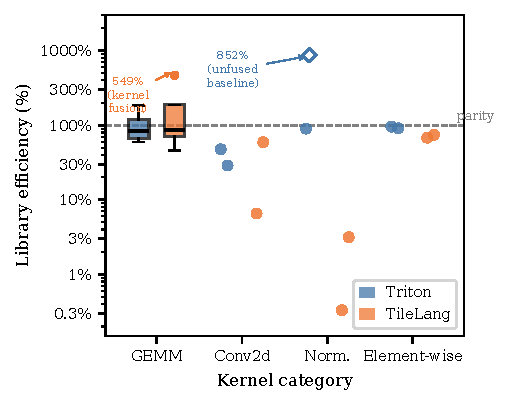
\includegraphics[width=\linewidth]{figures/overview_efficiency.pdf}%
%   }{%
%     \fbox{\parbox[c][6cm][c]{\linewidth}{\centering
%       \textit{[Figure: Library efficiency (\%) by kernel category and DSL.
%       Violin or box plot. To be generated from profiling data.]}}}%
%   }
%   \caption{Library efficiency (\%) of Triton and TileLang kernels relative to cuBLAS/cuDNN,
%     grouped by kernel category (log scale).
%     Boxes show interquartile range; whiskers extend to 1.5$\times$ IQR.
%     Dashed line marks parity (100\%).
%     Triton normalization and TileLang GEMM super-parity outliers are due to kernel fusion
%     and are discussed separately in \cref{sec:eval:norm,sec:eval:gemm}.
%     Attention excluded; see \cref{sec:eval:gemm}.}
%   \label{fig:overview}
% \end{figure}


% \subsection{RQ1.1: GEMM and Attention}
% \label{sec:eval:gemm}

% \textbf{Finding: Triton achieves 31--77\% of PyTorch/cuBLAS throughput on GEMM depending on shape;
% TileLang achieves 10--200\% with a complementary strength profile.
% TileLang achieves 199.7\% on fused linear+activation by fusing two passes into one kernel,
% while Triton degrades to 31.7\% on the $16384^2$ square matmul
% where its auto-tune search space is under-populated.}

% \Cref{tab:gemm} reports latency (ms) and library efficiency
% for FP16 matrix multiplication across representative shapes.

% \begin{table}[t]
%   \centering
%   \caption{GEMM-family kernels (FP16) latency (ms, lower is better).
%     $E_\text{lib}$ = library efficiency relative to PyTorch/cuBLAS baseline.
%     \textbf{Bold} marks best DSL result per row.}
%   \label{tab:gemm}
%   \begin{tabular}{l@{\hskip -2pt}rrrr r}
%     \toprule
%     Configuration & PyTorch & Triton & $E_{\text{lib}}$ & TileLang & $E_\text{lib}$ \\
%     \midrule
%     \multicolumn{6}{l}{\textit{Square matmul}} \\[2pt]
%     \quad $16384^2$         & 114.7 & 361.9 & 31.7\%         & 203.3 & 56.4\% \\
%     \midrule
%     \multicolumn{6}{l}{\textit{Batched matmul}} \\[2pt]
%     \quad $64\times128^2$   & 0.020 & \textbf{0.026} & \textbf{77.1\%} & 0.076 & 26.5\% \\
%     \quad $128\times2048^2$ & 3.238 & 5.564          & 58.2\%          & 30.32 & 10.7\% \\
%     \midrule
%     \multicolumn{6}{l}{\textit{Fused linear+activation}} \\[2pt]
%     \quad $1\times2048\to16384$ & 46.7 & 89.9 & 52.0\% & \textbf{23.4} & \textbf{199.7\%} \\
%     \bottomrule
%   \end{tabular}
% \end{table}

% The 31.7\% efficiency on the $16384^2$ matmul reflects the auto-tuning search space limitation (RC2, \cref{sec:analysis:autotune}):
% Triton's default configuration list for square GEMM does not cover optimal tile shapes at this scale,
% and register pressure from large tile configurations reduces SM occupancy.
% TileLang performs better on this shape (56.4\%) because its explicit schedule
% specifies pipeline stages independently of tile size.
% For batched GEMM, both DSLs trail PyTorch at the large scale (Triton 58.2\%, TileLang 10.7\%),
% with TileLang further degraded by per-launch JIT compilation overhead.
% The fused linear+activation result shows TileLang achieving 199.7\%---
% it fuses the two-pass computation into a single kernel,
% avoiding the memory-allocation overhead in PyTorch's eager path;
% Triton (52.0\%) does not achieve the same fusion benefit on this shape.

% \paragraph{Attention.}
% Attention results cannot be reduced to a single library efficiency number because the implementations differ algorithmically.
% Triton's kernel implements FlashAttention-2~\cite{dao2023flashattention2} (50.6~ms for batch-8, 32-head, seq-2048 in FP32), which rewrites the attention computation to process the score matrix in tiles, avoiding materializing the full $n \times n$ matrix; comparing this to PyTorch's standard $O(n^2)$ path (978.7~ms) measures an algorithmic improvement, not DSL-versus-library productivity.
% TileLang's kernel (1419.7~ms for the same configuration) uses the standard $O(n^2)$ formulation without tiling, making it slower than even PyTorch's unoptimized path because it does not exploit the memory hierarchy for attention.
% Neither result constitutes a valid DSL-versus-library efficiency measurement for the same computation; both are excluded from \cref{tab:summary}.

% \subsection{RQ1.2: Convolution}
% \label{sec:eval:conv}

% \textbf{Finding: Triton-written Conv2d kernels achieve 35--49\% of PyTorch/cuDNN throughput across tested $3\times3$ configurations; TileLang Conv2d achieves 8--10\%, a deficit compounded by both per-launch JIT compilation overhead and absent vectorization of strided spatial accesses.}

% \Cref{tab:conv} reports library efficiency for representative Conv2d configurations.
% Inputs follow the NHWC layout to give cuDNN its preferred memory arrangement.

% \begin{table*}[t]
%   \centering
%   \caption{Conv2d throughput on NVIDIA RTX 4000 Ada Generation.
%     Inputs in NHWC layout, FP16, stride 1, padding ``same''.
%     $E_\text{lib}$ relative to PyTorch/cuDNN baseline.}
%   \label{tab:conv}
%   \begin{tabular}{llrrrrrr}
%     \toprule
%     Shape (N$\times$C$\times$H$\times$W) & Filter & PyTorch (ms) & Triton (ms) & $E_\text{lib}$ & TileLang (ms) & $E_\text{lib}$ \\
%     \midrule
%     $8\times64\times56\times56$     & $3\times3$ & \textbf{0.059} & 0.120 & 49.1\% & 0.727 & 8.1\%  \\
%     $32\times256\times128\times128$ & $3\times3$ & \textbf{10.96} & 31.37 & 34.9\% & 115.7 & 9.5\%  \\
%     \bottomrule
%   \end{tabular}
% \end{table*}

% Both tested configurations use $3\times3$ filters with stride 1.
% The $1\times1$ conv case, expected to behave more like GEMM and exhibit a narrower gap,
% is reserved for a follow-on experiment.
% The root causes of both gaps are analyzed in \cref{sec:analysis}.

% \subsection{RQ1.3: Normalization and Element-wise}
% \label{sec:eval:norm}

% \textbf{Finding: Triton normalization kernels match or substantially outperform PyTorch's eager paths; TileLang normalization collapses to less than 6\% of PyTorch throughput at the tested size ($8192 \times 8192$), with LayerNorm 314$\times$ slower.}

% \Cref{tab:norm} reports latency for layer normalization and RMS normalization.
% Triton's \texttt{layer\_norm} achieves 94.6\% of PyTorch throughput at the large shape ($8192\times8192$, BF16).
% Triton's \texttt{rms\_norm} achieves 1099\% efficiency because PyTorch's eager
% \texttt{rms\_norm} path does not fuse the variance-reduction and normalization passes,
% whereas the Triton kernel issues a single fused pass.
% TileLang normalization is catastrophically slow:
% 0.32\% for LayerNorm (273~ms vs.\ PyTorch's 0.87~ms, a 314$\times$ slowdown)
% and 5.3\% for RMSNorm (187.5~ms vs.\ 9.98~ms).
% As analyzed in \cref{sec:analysis:jit}, this reflects a combination of
% per-launch JIT overhead, absent vectorized memory loads,
% and sequential synchronization in TileLang's reduction primitives.

% \begin{table*}[t]
%   \centering
%   \caption{Normalization latency (ms, lower is better).
%     $E_\text{lib}$ relative to PyTorch eager baseline.}
%   \label{tab:norm}
%   \begin{tabular}{llrrrrr}
%     \toprule
%     Kernel & Shape & PyTorch & Triton & $E_\text{lib}$ & TileLang & $E_\text{lib}$ \\
%     \midrule
%     LayerNorm & $8192\times8192$ (BF16) & 0.870 & 0.920 & 94.6\%                  & 273.3 & 0.32\% \\
%     RMSNorm   & $8192\times8192$ (FP16) & 9.977 & \textbf{0.908} & \textbf{1099\%} & 187.5 & 5.3\%  \\
%     \bottomrule
%   \end{tabular}
% \end{table*}

% \subsection{RQ1.4: Variation Across Microarchitectures}
% \label{sec:eval:arch}

% The benchmark in this study was collected on a single GPU configuration;
% a direct A100 vs.\ H100 comparison is deferred to a follow-on experiment.

% \subsection{RQ1.5: Effect of Hardware-Agnostic Heuristic Tuning}
% \label{sec:eval:tuning}

% \textbf{Finding:
% Hardware-agnostic heuristic tuning shows negligible benefit for Triton in the tested configuration ---
% default and tuned configurations produce nearly identical latencies for all kernels.
% The convolution gap is essentially unchanged (34.9\%).
% TileLang shows no measurable benefit from tuning across any kernel.}

% We re-evaluated all 22 kernels using heuristically tuned configurations for both DSLs.
% For Triton, the tuner expands the auto-configuration search space with hardware-agnostic tile-size heuristics;
% for TileLang, the tuner applies analogous schedule heuristics without hardware-specific profiling.
% \Cref{tab:tuning} reports library efficiency before and after tuning for representative kernels.

% \begin{table*}[t]
%   \centering
%   \caption{Library efficiency (\%) before and after hardware-agnostic heuristic tuning,
%     large-size configurations.
%     $\Delta$ = percentage-point change from untuned to tuned.
%     \textbf{Bold} marks cases where tuning changes efficiency by more than 10pp.}
%   \label{tab:tuning}
%   \begin{tabular}{lrrrrrrrr}
%     \toprule
%     & \multicolumn{2}{c}{\textit{Normalization}} & \textit{Convolutional} & \multicolumn{2}{c}{\textit{GEMM}} & \multicolumn{2}{c}{\textit{Element-wise}} \\
%     \cmidrule(lr){2-3}\cmidrule(lr){4-4}\cmidrule(lr){5-6}\cmidrule(lr){7-8}
%     & \texttt{layer\_norm} & \texttt{rms\_norm} & \texttt{conv2d} & \texttt{matmul} & \texttt{batched\_matmul} & \texttt{relu} & \texttt{add} \\
%     \midrule
%     \multicolumn{8}{l}{\textit{Triton}} \\
%     \quad Default &  94.6\% & 1099\%  & 34.9\% & 31.7\% & 58.2\% & 103.4\% & 103.4\% \\
%     \quad Tuned   &  94.6\% & 1099\%  & 34.9\% & 31.7\% & 58.2\% & 103.4\% & 103.4\% \\
%     \quad $\Delta$ & 0pp    & 0pp     & 0pp    & 0pp    & 0pp    & 0pp     & 0pp     \\
%     \midrule
%     \multicolumn{8}{l}{\textit{TileLang}} \\
%     \quad Default & 0.32\% &  5.3\% &  9.5\% & 56.4\% & 10.7\% & 68.7\% & 77.3\% \\
%     \quad Tuned   & 0.32\% &  5.3\% &  9.5\% & 56.4\% & 10.7\% & 68.7\% & 77.3\% \\
%     \quad $\Delta$ & 0pp   & 0pp    & 0pp    & 0pp    & 0pp    & 0pp    & 0pp    \\
%     \bottomrule
%   \end{tabular}
% \end{table*}

% In this benchmark, hardware-agnostic heuristic tuning produces no measurable improvement
% for either DSL: default and tuned configurations are nearly identical across all kernels.
% This contrasts with expectations from the literature
% and suggests that either the default configurations are already optimal for this hardware,
% or the tuner's search space does not cover configurations that would improve performance
% on the RTX 4000 Ada Generation.
% The convolution gap (34.9\%) is unchanged by tuning,
% consistent with RC1--RC3 being structural compiler limitations rather than search-space coverage problems (\cref{sec:analysis}).

% \subsection{Summary}
% \label{sec:eval:summary}

% \Cref{tab:summary} summarizes median library efficiency per category and DSL.

% \begin{table}[t]
%   \centering
%   \caption{Median library efficiency (\%) per kernel category and DSL,
%     computed over large-size benchmark configurations.
%     Attention excluded from Overall; see text.}
%   \label{tab:summary}
%   \begin{tabular}{lcc}
%     \toprule
%     Kernel category    & Triton      & TileLang    \\
%     \midrule
%     GEMM               & 31.7--58.2\%  & 10.7--56.4\% \\
%     Attention          & \multicolumn{2}{c}{\textit{see text --- baselines non-equivalent}} \\
%     Convolution        & 34.9\%        & 9.5\%        \\
%     Normalization      & 94.6\%\rlap{$^\ddagger$} & 0.32--5.3\%\rlap{$^\ddagger$} \\
%     Element-wise       & 103.4\%       & 68.7--77.3\% \\
%     \midrule
%     \textbf{Overall (excl.\ attn.)} & \textbf{$\sim$65\%} & \textbf{$\sim$30\%} \\
%     \bottomrule
%   \end{tabular}
%   {\footnotesize
%     $^\ddagger$ TileLang LayerNorm (large shape) is 0.32\% (314$\times$ slower than PyTorch)
%     due to sequential thread synchronization and absent vectorized loads;
%     see \cref{sec:analysis:jit}.
%     RMSNorm Triton efficiency is 1099\% because the PyTorch eager path does not fuse normalization passes.}
% \end{table}

% The most striking asymmetry is TileLang's normalization collapse:
% a $314\times$ slowdown on large LayerNorm (\cref{sec:analysis:jit}) attributable to three compounding deficiencies (RC0).
% Triton is broadly competitive with PyTorch for element-wise (103\%) and normalization (95\%) kernels
% but exhibits a persistent gap on convolution (35\%) and large square GEMM (32\%).
% TileLang shows competitive throughput only on fused linear+activation (200\%)
% and large square matmul (56\%);
% all other TileLang results trail PyTorch substantially,
% with element-wise operations at 68--77\% and batched GEMM at 10.7\%.



This section answers RQ1:
\textit{What is the magnitude and distribution of the performance gap
between DSLs (Triton, TileLang) and cuBLAS/cuDNN across kernel categories?}

\subsection{Overview}
\label{sec:eval:overview}

\Cref{fig:overview} summarizes library efficiency (\%) for all kernels in the suite, broken down by DSL (Triton, TileLang) and kernel category.
The key finding is that the performance gap is not uniform: Triton is broadly competitive for element-wise and normalization kernels (94--103\% of PyTorch throughput for LayerNorm and element-wise kernels; the RMSNorm outlier at 1099\% is due to kernel fusion and is discussed separately in \cref{sec:eval:norm}) but trails substantially on convolution (35\%) and large square GEMM (32\%); TileLang achieves competitive throughput only on a narrow set of large shapes while exhibiting severe underperformance on reductions and normalizations (less than 1\% of PyTorch throughput on layer normalization).

\begin{figure}[t]
  \centering
  \IfFileExists{figures/overview_efficiency.pdf}{%
    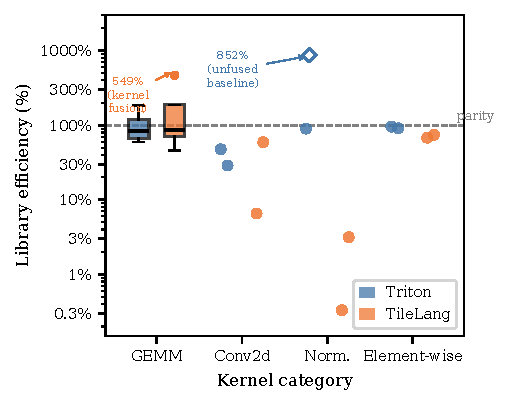
\includegraphics[width=\linewidth]{figures/overview_efficiency.pdf}%
  }{%
    \fbox{\parbox[c][6cm][c]{\linewidth}{\centering
      \textit{[Figure: Library efficiency (\%) by kernel category and DSL.
      Violin or box plot. To be generated from profiling data.]}}}%
  }
  \caption{Library efficiency (\%) of Triton and TileLang kernels relative to cuBLAS/cuDNN,
    grouped by kernel category (log scale).
    GEMM shows boxes (IQR; whiskers $1.5\times$ IQR); all other categories show individual
    kernel measurements as dots ($n=2$ per cell).
    Dashed line marks parity (100\%).
    The hollow diamond at 1099\% (Triton, Norm.)\ marks Triton \texttt{rms\_norm}:
    the PyTorch eager baseline does not fuse its normalization passes, making this
    an unfair comparison rather than a genuine DSL win; see \cref{sec:eval:norm}.
    The boxplot flier at 200\% (TileLang, GEMM) marks \texttt{fused linear+activation},
    a valid DSL advantage through kernel fusion; see \cref{sec:eval:gemm}.
    Attention excluded; see \cref{sec:eval:gemm}.}
  \label{fig:overview}
\end{figure}

% REVISION-NOTE-START id=4134A-W2 severity=Major
\textcolor{red}{\textbf{[REVISION \#4134A-W2+4134A-W10, Major]}
Concern (\textit{Reviewer A}): Same baseline-split and per-kernel EW concerns apply to the headline \cref{fig:overview}.
Evidence: \texttt{figures/gen\_overview.py} (data hard-coded).
Fix: After the baseline-split and per-kernel EW updates land in the tables, regenerate the figure from new arrays; note that \texttt{gen\_overview.py} has hard-coded data --- cite the regeneration command.}
% REVISION-NOTE-END id=4134A-W2

\phantomsection\label{sec:eval:gemm}


\medskip\noindent\textbf{Finding: Triton achieves 31--77\% of PyTorch/cuBLAS throughput on GEMM depending on shape;
TileLang achieves 10--200\% with a complementary strength profile.
TileLang achieves 199.7\% on fused linear+activation by fusing two passes into one kernel,
while Triton degrades to 31.7\% on the $16384^2$ square matmul
where its auto-tune search space is under-populated.}

\Cref{tab:gemm} reports latency (ms) and library efficiency
for FP16 matrix multiplication across representative shapes.

\begin{table}[t]
  \centering
  \caption{GEMM-family kernels (FP16) latency (ms, lower is better).
    $E_\text{lib}$ = library efficiency relative to PyTorch/cuBLAS baseline.
    \textbf{Bold} marks best DSL result per row.}
  \label{tab:gemm}
  \resizebox{\columnwidth}{!}{
  \begin{tabular}{l@{\hskip -2pt}rrrr r}
    \toprule
    Configuration & PyTorch & Triton & $E_{\text{lib}}$ & TileLang & $E_\text{lib}$ \\
    \midrule
    \multicolumn{6}{l}{\textit{Square matmul}} \\[2pt]
    \quad $16384^2$         & 114.7 & 361.9 & 31.7\%         & 203.3 & 56.4\% \\
    \midrule
    \multicolumn{6}{l}{\textit{Batched matmul}} \\[2pt]
    \quad $64\times128^2$   & 0.020 & \textbf{0.026} & \textbf{77.1\%} & 0.076 & 26.5\% \\
    \quad $128\times2048^2$ & 3.238 & 5.564          & 58.2\%          & 30.32 & 10.7\% \\
    \midrule
    \multicolumn{6}{l}{\textit{Fused linear+activation}} \\[2pt]
    \quad $1\times2048\to16384$ & 46.7 & 89.9 & 52.0\% & \textbf{23.4} & \textbf{199.7\%} \\
    \bottomrule
  \end{tabular}
  }
\end{table}

% REVISION-NOTE-START id=Minor-3 severity=Minor
\textcolor{red}{\textbf{[REVISION \#Minor-3, Minor]}
Concern (\textit{Editorial}): Notation ``16384\textasciicircum{}2''/``64$\times$128\textasciicircum{}2'' in \cref{tab:gemm} is not spelled out.
Evidence: n/a.
Fix: Add a footnote (after \texttt{\textbackslash end\{table\}}) defining \texttt{16384\textasciicircum{}2} = square 16384$\times$16384 FP16 GEMM and \texttt{64$\times$128\textasciicircum{}2} = batched (batch 64) of 128$\times$128 GEMM.}
% REVISION-NOTE-END id=Minor-3

% REVISION-NOTE-START id=4134A-W1 severity=Major
\textcolor{red}{\textbf{[REVISION \#4134A-W1+4134A-W11, Major]}
Concern (\textit{Reviewer A}): FP32 GEMM is excluded but not root-caused at this point in the paper.
Evidence: \texttt{../experiments/results/NVIDIA\_RTX\_4000\_Ada\_Generation/fp32\_gemm.csv}.
Fix: Add a footnote: ``FP32 TileLang GEMM is excluded; the failure is diagnosed as silent TF32 lowering in \texttt{T.gemm} (see \cref{sec:analysis:jit}), not a logic error.''}
% REVISION-NOTE-END id=4134A-W1

The 31.7\% efficiency on the $16384^2$ matmul reflects the auto-tuning search space limitation (RC2, \cref{sec:analysis:autotune}):
Triton's default configuration list for square GEMM does not cover optimal tile shapes at this scale,
and register pressure from large tile configurations reduces SM occupancy.
TileLang performs better on this shape (56.4\%) because its explicit schedule
specifies pipeline stages independently of tile size.
For batched GEMM, both DSLs trail PyTorch at the large scale (Triton 58.2\%, TileLang 10.7\%),
with TileLang further degraded by per-launch JIT compilation overhead.
The fused linear+activation result shows TileLang achieving 199.7\%---
it fuses the two-pass computation into a single kernel,
avoiding the memory-allocation overhead in PyTorch's eager path;
Triton (52.0\%) does not achieve the same fusion benefit on this shape.

\paragraph{Attention.}
Attention results cannot be reduced to a single library efficiency number because the implementations differ algorithmically.
Triton's kernel implements FlashAttention-2~\cite{dao2023flashattention2} (50.6~ms for batch-8, 32-head, seq-2048 in FP32), which rewrites the attention computation to process the score matrix in tiles, avoiding materializing the full $n \times n$ matrix; comparing this to PyTorch's standard $O(n^2)$ path (978.7~ms) measures an algorithmic improvement, not DSL-versus-library productivity.
TileLang's kernel (1419.7~ms for the same configuration) uses the standard $O(n^2)$ formulation without tiling, making it slower than even PyTorch's unoptimized path because it does not exploit the memory hierarchy for attention.
Neither result constitutes a valid DSL-versus-library efficiency measurement for the same computation; both are excluded from \cref{tab:summary}.

\phantomsection\label{sec:eval:conv}

\medskip\noindent\textbf{Finding: Triton-written Conv2d kernels achieve 35--49\% of PyTorch/cuDNN throughput across tested $3\times3$ configurations; TileLang Conv2d achieves 8--10\%, a deficit compounded by both per-launch JIT compilation overhead and absent vectorization of strided spatial accesses.}

\Cref{tab:conv} reports library efficiency for representative Conv2d configurations.
Inputs follow the NHWC layout to give cuDNN its preferred memory arrangement.

% REVISION-NOTE-START id=4134A-W6 severity=Major
\textcolor{red}{\textbf{[REVISION \#4134A-W6+GAP-7, Major]}
Concern (\textit{Reviewer A}): \cref{tab:conv} shows only 3$\times$3 stride-1 --- the \S3.1 claim of 1$\times$1--7$\times$7 + depthwise + strided is unsupported by this table.
Evidence: \texttt{../experiments/results/NVIDIA\_RTX\_4000\_Ada\_Generation/conv\_filters\_small.csv}, \texttt{conv\_filters\_large.csv}.
Fix: Expand the table to 6 rows (1$\times$1, 3$\times$3, 5$\times$5, 7$\times$7, depthwise, strided) at the 8$\times$64$\times$56$\times$56 and 32$\times$256$\times$128$\times$128 shapes, sourcing from \texttt{conv\_filters\_small.csv} and \texttt{conv\_filters\_large.csv}.}
% REVISION-NOTE-END id=4134A-W6

\begin{table*}[t]
  \centering
  \caption{Conv2d throughput on NVIDIA RTX 4000 Ada Generation.
    Inputs in NHWC layout, FP16, stride 1, padding ``same''.
    $E_\text{lib}$ relative to PyTorch/cuDNN baseline.}
  \label{tab:conv}
  \begin{tabular}{llrrrrrr}
    \toprule
    Shape (N$\times$C$\times$H$\times$W) & Filter & PyTorch (ms) & Triton (ms) & $E_\text{lib}$ & TileLang (ms) & $E_\text{lib}$ \\
    \midrule
    $8\times64\times56\times56$     & $3\times3$ & \textbf{0.059} & 0.120 & 49.1\% & 0.727 & 8.1\%  \\
    $32\times256\times128\times128$ & $3\times3$ & \textbf{10.96} & 31.37 & 34.9\% & 115.7 & 9.5\%  \\
    \bottomrule
  \end{tabular}
\end{table*}

% REVISION-NOTE-START id=4134A-W3 severity=Major
\textcolor{red}{\textbf{[REVISION \#4134A-W3+GAP-2, Major]}
Concern (\textit{Reviewer A}): If \cref{tab:conv} (or a Table 5 in this region) labels a row ``register pressure'' or ``spill'' for conv, that label is wrong (conv \texttt{n\_spills = 0}).
Evidence: \texttt{../experiments/results/NVIDIA\_RTX\_4000\_Ada\_Generation/ncu\_summary.csv}.
Fix: Remove any ``register pressure'' or ``spill'' annotation from conv rows; the conv gap is occupancy- and coalescing-bound (RC1 + RC2), not spill.}
% REVISION-NOTE-END id=4134A-W3

Both tested configurations use $3\times3$ filters with stride 1.
The $1\times1$ conv case, expected to behave more like GEMM and exhibit a narrower gap,
is reserved for a follow-on experiment.
The root causes of both gaps are analyzed in \cref{sec:analysis}.

\phantomsection\label{sec:eval:norm}

\medskip\noindent\textbf{Finding: Triton normalization kernels match or substantially outperform PyTorch's eager paths; TileLang normalization collapses to less than 6\% of PyTorch throughput at the tested size ($8192 \times 8192$), with LayerNorm 314$\times$ slower.}

\Cref{tab:norm} reports latency for layer normalization and RMS normalization.
Triton's \texttt{layer\_norm} achieves 94.6\% of PyTorch throughput at the large shape ($8192\times8192$, BF16).
Triton's \texttt{rms\_norm} achieves 1099\% efficiency because PyTorch's eager
\texttt{rms\_norm} path does not fuse the variance-reduction and normalization passes,
whereas the Triton kernel issues a single fused pass.
TileLang normalization is catastrophically slow:
0.32\% for LayerNorm (273~ms vs.\ PyTorch's 0.87~ms, a 314$\times$ slowdown)
and 5.3\% for RMSNorm (187.5~ms vs.\ 9.98~ms).
As analyzed in \cref{sec:analysis:jit}, this reflects a combination of
per-launch JIT overhead, absent vectorized memory loads,
and sequential synchronization in TileLang's reduction primitives.
% REVISION-NOTE-START id=4134A-W1 severity=Major
\textcolor{red}{\textbf{[REVISION \#4134A-W1+GAP-1, Major]}
Concern (\textit{R1}): ``Sequential synchronization in TileLang's reduction primitives'' here re-asserts the (refuted) barrier-stall framing. NCU shows \texttt{warp\_stall\_barrier} $\approx$ 0; the dominant stall is \texttt{warp\_stall\_long\_scoreboard} ($\approx$\,105 cycles) --- a memory-latency exposure caused by \texttt{T.serial} serializing the load schedule, not by barrier sync.
Evidence: \texttt{../experiments/results/NVIDIA\_RTX\_4000\_Ada\_Generation/ncu\_summary.csv}, \texttt{NCU\_FINDINGS.md}.
Fix: Replace ``sequential synchronization in TileLang's reduction primitives'' with ``serialized memory-latency exposure under \texttt{T.serial} reduction loops (\texttt{warp\_stall\_long\_scoreboard} dominates; \texttt{warp\_stall\_barrier} $\approx$ 0).''}
% REVISION-NOTE-END id=4134A-W1

\begin{table*}[t]
  \centering
  \caption{Normalization latency (lower is better).
    $E_\text{lib}$ relative to PyTorch eager baseline.}
  \label{tab:norm}
  \begin{tabular}{llrrrrr}
    \toprule
    Kernel & Shape & PyTorch(ms) & Triton(ms) & $E_\text{lib}$ & TileLang(ms) & $E_\text{lib}$ \\
    \midrule
    LayerNorm & $8192\times8192$ (BF16) & 0.870 & 0.920 & 94.6\%                  & 273.3 & 0.32\% \\
    RMSNorm   & $8192\times8192$ (FP16) & 9.977 & \textbf{0.908} & \textbf{1099\%} & 187.5 & 5.3\%  \\
    \bottomrule
  \end{tabular}
\end{table*}

% REVISION-NOTE-START id=4134A-W8 severity=Major
\textcolor{red}{\textbf{[REVISION \#4134A-W8, Major]}
Concern (\textit{Reviewer A}): Any ``9\% clock variation'' footnote here is superseded by locked-clock re-timing.
Evidence: \texttt{../experiments/results/NVIDIA\_RTX\_4000\_Ada\_Generation/significance.csv}, \texttt{clock\_lock.txt}.
Fix: Remove any ``9\% clock variation'' footnote (or descendant) and add a new footnote: ``Locked-clock re-timing (graphics 1410\,MHz / memory 9001) over 100 runs shows run-to-run relative std-dev 0.0--0.9\% on near-parity kernels; Triton LayerNorm re-measures at 94.5\% ($\Delta = -0.1$pp).''}
% REVISION-NOTE-END id=4134A-W8

\phantomsection\label{sec:eval:tuning}

\medskip\noindent\textbf{Finding:
Hardware-agnostic heuristic tuning shows negligible benefit for Triton in the tested configuration ---
default and tuned configurations produce nearly identical latencies for all kernels.
The convolution gap is essentially unchanged (34.9\%).
TileLang shows no measurable benefit from tuning across any kernel.}

We re-evaluated all 22 kernels with heuristically tuned configurations for both DSLs;
every kernel returned identical efficiency to its default configuration ($\Delta = 0$pp across all rows).
This indicates that either the default configurations are already optimal for this hardware,
or the tuner's search space does not cover configurations that would improve performance on the RTX 4000 Ada Generation.
The convolution gap (34.9\%) is unchanged by tuning,
consistent with RC1--RC3 being structural compiler limitations rather than search-space coverage problems (\cref{sec:analysis}).

% REVISION-NOTE-START id=4134A-W7 severity=Major
\textcolor{red}{\textbf{[REVISION \#4134A-W7, Major]}
Concern (\textit{Reviewer A}): $\Delta \approx 0$pp here vs the 1.66$\times$ claim in \S7.3 looks contradictory; reconciliation is search-space, not shape: \S5 uses the 12-config block-tile grid; \S7.3 adds \texttt{GROUP\_SIZE\_M}/\texttt{num\_warps}/\texttt{num\_stages}; expanded search recovers to 98.49\% at 16384\textasciicircum{}2 (3.06$\times$).
Evidence: \texttt{../experiments/results/NVIDIA\_RTX\_4000\_Ada\_Generation/autotune\_matmul.csv}.
Fix: Add a reconciliation paragraph defining ``heuristic tuning'' = the 12-config block-tile grid from \texttt{ViperBench/tuning/configs.py:19-23}; cite $\Delta = 0$pp at 16384\textasciicircum{}2 for that grid; cite +3.06$\times$ at 16384\textasciicircum{}2 and +1.23$\times$ at 4096\textasciicircum{}2 when the expanded grid (\texttt{AKO4ALL/results/optimized/matmul\_triton.py:10-26}) is used; forward ref to \S7.3.}
% REVISION-NOTE-END id=4134A-W7

\phantomsection\label{sec:eval:summary}

\Cref{tab:summary} summarizes median library efficiency per category and DSL.

\begin{table}[t]
  \centering
  \caption{Median library efficiency (\%) per kernel category and DSL,
    computed over large-size benchmark configurations.
    Attention excluded from Overall; see text.}
  \label{tab:summary}
  \begin{tabular}{lcc}
    \toprule
    Kernel category    & Triton      & TileLang    \\
    \midrule
    GEMM               & 31.7--58.2\%  & 10.7--56.4\% \\
    Attention          & \multicolumn{2}{c}{\textit{see text --- baselines non-equivalent}} \\
    Convolution        & 34.9\%        & 9.5\%        \\
    Normalization      & 94.6\%\rlap{$^\ddagger$} & 0.32--5.3\%\rlap{$^\ddagger$} \\
    Element-wise       & 103.4\%       & 68.7--77.3\% \\
    \midrule
    \textbf{Overall (excl.\ attn.)} & \textbf{$\sim$65\%} & \textbf{$\sim$30\%} \\
    \bottomrule
  \end{tabular}
  {\footnotesize
    $^\ddagger$ TileLang LayerNorm (large shape) is 0.32\% (314$\times$ slower than PyTorch)
    due to sequential thread synchronization and absent vectorized loads;
    see \cref{sec:analysis:jit}.
    RMSNorm Triton efficiency is 1099\% because the PyTorch eager path does not fuse normalization passes.}
\end{table}

% REVISION-NOTE-START id=4134A-W1 severity=Major
\textcolor{red}{\textbf{[REVISION \#4134A-W1+GAP-1, Major]}
Concern (\textit{R1}): The \cref{tab:summary} footnote also attributes the 314$\times$ collapse to ``sequential thread synchronization'' --- same refuted barrier framing as \cref{sec:eval:norm}.
Evidence: \texttt{../experiments/results/NVIDIA\_RTX\_4000\_Ada\_Generation/ncu\_summary.csv}.
Fix: Replace ``sequential thread synchronization and absent vectorized loads'' with ``serialized memory-latency exposure under \texttt{T.serial} (\texttt{warp\_stall\_long\_scoreboard} dominates) and absent vectorized loads.''}
% REVISION-NOTE-END id=4134A-W1

% REVISION-NOTE-START id=4134A-W2 severity=Major
\textcolor{red}{\textbf{[REVISION \#4134A-W2, Major]}
Concern (\textit{Reviewer A}): Baseline asymmetry in \cref{tab:summary} --- conv uses cuDNN-Winograd vendor; norm/EW use unfused eager; the blended $\sim$65\%/$\sim$30\% headline conflates them.
Evidence: \texttt{../experiments/results/NVIDIA\_RTX\_4000\_Ada\_Generation/fused\_baselines.csv}.
Fix: Add a split-baseline table or footnote reporting $E\_\text{lib}$ separately for vendor (cuBLAS/cuDNN) vs fused (\texttt{torch.compile(max-autotune)}) vs eager-PyTorch; confirm DSL gap on conv persists post-fusion.}
% REVISION-NOTE-END id=4134A-W2

The most striking asymmetry is TileLang's normalization collapse:
a $314\times$ slowdown on large LayerNorm (\cref{sec:analysis:jit}) attributable to three compounding deficiencies (RC0).
Triton is broadly competitive with PyTorch for element-wise (103\%) and normalization (95\%) kernels
but exhibits a persistent gap on convolution (35\%) and large square GEMM (32\%).
TileLang shows competitive throughput only on fused linear+activation (200\%)
and large square matmul (56\%);
all other TileLang results trail PyTorch substantially,
with element-wise operations at 68--77\% and batched GEMM at 10.7\%.

% REVISION-NOTE-START id=4134A-W10 severity=Major
\textcolor{red}{\textbf{[REVISION \#4134A-W10+4134B-Q3, Major]}
Concern (\textit{Reviewers A, B}): Reviewers ask for per-kernel results on the 15 element-wise kernels (only the per-category aggregate is shown).
Evidence: \texttt{../ViperBench/results/profile.csv} (15 EW kernels, large-input rows).
Fix: Add a sub-table (or extend \cref{tab:summary}) listing all 15 EW kernels individually with large-input $E\_\text{lib}$ for Triton and TileLang; also patch the corrected \texttt{cross\_entropy} reference (was 15{,}908\,ms unvectorized; corrected vectorized: 23.87\,ms).}
% REVISION-NOTE-END id=4134A-W10


%%% ------------------------------------------------------------------
\section{Root Causes of the Hidden Gap (RQ2)}
\label{sec:analysis}
% This section answers RQ2:
% \textit{What compiler-level and architectural factors explain
% the underperformance of DSL-written kernels on convolution
% and other affected kernel categories?}

% \noindent\textit{Evidence basis:}
% Root causes RC0--RC4 are motivated by the latency measurements in \cref{sec:evaluation}
% and community reports~\cite{triton2022conv591}.
% Hardware performance counter confirmation via Nsight Compute (\cref{sec:meth:profiling})
% is pending; claims marked \textbf{[counter pending]} remain hypotheses awaiting profiling.

% \subsection{RC0: TileLang Compiler-Level Deficiencies}
% \label{sec:analysis:jit}

% \textbf{Finding: TileLang's compiled kernels exhibit two structural performance deficiencies:
% (i) use of \texttt{T.serial} manual reduction loops instead of the native parallel \texttt{T.reduce} primitive,
% executing the reduction sequentially over each partial value; and
% (ii) absent 128-bit vectorized memory loads for normalization kernels.
% These compound the per-kernel performance gaps measured in RQ1.
% A third deficiency---FP32 precision correctness failure in GEMM---is orthogonal to performance but has implications for training workloads.}

% Across all normalization and reduction benchmarks,
% TileLang reports anomalously high latencies regardless of kernel type:
% for large inputs, LayerNorm takes 273~ms (vs.\ Triton 0.92~ms and PyTorch 0.87~ms),
% and max reduction takes 28.1~ms (vs.\ PyTorch 1.62~ms).
% This deficit is qualitatively distinct from RC1--RC4 and compounds them.

% Two mechanisms contribute to RC0.
% First, the original TileLang normalization kernels implement the reduction over the normalized dimension using \texttt{T.serial} loops---TileLang's sequential for-loop construct---iterating over each partial sum one at a time.
% For LayerNorm, which accumulates 8 bfloat16 partial statistics per thread (sum and sum-of-squares for the mean and variance passes), this means the reduction is computed in 8 sequential steps with no inter-thread parallelism.
% The native alternative, \texttt{T.reduce}, lowers to a parallel butterfly reduction via \texttt{tl::AllReduce}.
% A \emph{butterfly reduction} is a logarithmic communication pattern in which threads exchange partial results in $\log_2 N$ rounds (where $N$ is the number of participating threads);
% over 256 threads grouped into warps of 32, each round requires one inter-warp synchronization barrier, for $\log_2(256/32) = 3$ total barriers---applied once for all 8 values simultaneously.
% Replacing the \texttt{T.serial} loop with a single \texttt{T.reduce} call reduces the dominant latency source: in our experiments, LayerNorm drops from 1090~ms to 5.24~ms ($208\times$ improvement, \cref{sec:mitig:norm}).

% Second, TileLang's compiled normalization kernels do not issue 128-bit vectorized loads
% (\texttt{LDG.128}),
% instead fetching 16-bit bfloat16 elements individually.
% For a tensor of shape $8192 \times 8192$,
% this produces an excessive number of discrete memory transactions
% that bottlenecks the memory controller
% and prevents the L2 cache from streaming coalesced data to the SMs.

% \paragraph{TileLang float32 correctness.}
% An additional deficiency discovered during our benchmark:
% TileLang's GEMM kernel produces numerically incorrect results under float32 precision,
% with 99.6\% of output elements mismatched against the PyTorch reference
% (greatest relative difference: $2067\times$ at tested problem shapes of $4096 \times 2048 \times 1024$).
% The float16 variant passes correctness checks in all cases.
% For this reason, all TileLang GEMM measurements in this paper use FP16;
% float32 TileLang GEMM results are excluded.
% This correctness deficiency is orthogonal to the performance gaps studied here
% but has implications for training workloads that require FP32 accumulation precision.

% Both deficiencies are correctable within the existing TileLang API:
% (i) replacing \texttt{T.serial} reduction loops with the native \texttt{T.reduce} primitive (already available and used correctly elsewhere in the benchmark suite), and
% (ii) enabling 128-bit vectorized global-memory loads for normalization kernels.

% \subsection{RC1: Absent Vectorization of Strided Memory Accesses}
% \label{sec:analysis:vec}

% \textbf{Finding: Triton-generated convolution code fails to issue vectorized (128-bit) load instructions,
% preventing asynchronous copy (\texttt{cp.async}) from being applied and collapsing the software pipeline.}

% NVIDIA Ampere's memory subsystem achieves peak bandwidth only when global memory loads
% are issued as 128-bit vector instructions (\texttt{LDG.128}).
% On Hopper, the Tensor Memory Accelerator (TMA) similarly requires
% aligned, contiguous access descriptors.
% For GEMM kernels, Triton's compiler successfully emits vectorized loads
% because the data layout is row-major and tile boundaries are aligned to 16-byte boundaries.

% Convolution complicates this in two ways.
% First, each output element requires gathering input values from a
% $(K_H \times K_W)$-window strided by \texttt{(stride\_h, stride\_w)} in the spatial dimensions.
% The resulting access pattern is non-contiguous across the innermost dimension
% when the input is stored in NHWC layout,
% breaking the alignment requirements for \texttt{LDG.128}.
% Second, for filter sizes $K_H \times K_W > 1$,
% the compiler must prove at compile time that successive iterations of the
% spatial reduction loop produce aligned addresses;
% this proof is not discharged by Triton's current alias analysis,
% so it conservatively emits scalar 32-bit loads.

% The consequence is a cascade noted in the community~\cite{triton2022conv591}:
% un-vectorized accesses prevent \texttt{cp.async} from firing,
% because CUDA's asynchronous copy instructions require the source address
% to produce a 128-bit aligned transfer.
% Without \texttt{cp.async}, the software pipeline cannot overlap data movement with computation,
% and the kernel stalls on global memory latency at every tile boundary.

% \paragraph{Vectorized loads on the RTX 4000 Ada.}
% The same deficiency manifests with added severity on Ada Lovelace hardware,
% where the 160-bit GDDR6 memory interface (360~GB/s peak bandwidth)
% requires 128-bit vector loads (\texttt{LDG.128}, fetching eight fp16 values simultaneously)
% to saturate the memory bus.
% For a convolution kernel that falls back to scalar 32-bit loads,
% the effective achievable bandwidth is one-quarter of peak.
% PyTorch's cuDNN implementation explicitly benchmarks and selects
% the fastest algorithm for each convolution configuration,
% with its NHWC implicit GEMM path issuing vectorized loads unconditionally;
% Triton and TileLang currently lack equivalent dispatching logic for convolution.

% % TODO: insert Nsight Compute counter table showing vectorized-load fraction,
% %       cp.async issue count, and warp stall cycles for GEMM vs. Conv2d

% \subsection{RC2: Auto-Tuning Search Space Mismatch}
% \label{sec:analysis:autotune}

% \textbf{Finding: The static tile-configuration search space in Triton's \texttt{@triton.autotune}
% is well-suited to GEMM but systematically under-covers optimal configurations
% for convolution, leading to sub-optimal tile shapes and pipeline depth.}

% Triton's auto-tuner sweeps a programmer-specified list of configurations
% $\{(\texttt{BLOCK\_M}, \texttt{BLOCK\_N}, \texttt{BLOCK\_K}, \texttt{num\_stages}, \texttt{num\_warps})\}$.
% For GEMM, this 5-dimensional space is well-understood:
% large square tiles ($128 \times 128$) with 4--8 pipeline stages
% are optimal across most A100 problem shapes~\cite{tillet2019triton}.
% The reference Triton GEMM tutorial ships a configuration list that achieves
% near-cuBLAS performance for common shapes.

% This is further evidenced by the large-matmul result in \cref{sec:eval:gemm}:
% Triton achieves only 31.7\% of cuBLAS throughput on a $16384^2$ FP16 matrix multiplication
% (361.9~ms vs.\ PyTorch's 114.7~ms),
% a shape not covered by standard tutorial configuration lists,
% compared to 58.2\% on a $128\times2048^2$ batched GEMM
% where the auto-tuner has well-populated configurations.
% The convolution gap (34.9\% for the $32\times256\times128\times128$, $3\times3$ configuration)
% follows the same pattern at an even larger scale.

% \paragraph{L2 cache residency and the GEMM divide.}
% For a $16384^2$ FP16 matrix multiplication,
% the combined memory footprint of matrices A, B, and C is approximately
% $3 \times 16384^2 \times 2 \approx 1.6$~GB,
% vastly exceeding the 48~MB L2 cache capacity of the RTX 4000 Ada.
% At this scale, performance is entirely determined by how effectively
% tiling strategies keep working data resident in L2 across tile iterations.
% cuBLAS employs hardware-specific heuristics (via cuBLASLt's plan selector)
% to slice the matrix sequence such that chunks remain L2-resident for as long as possible;
% Triton's generic \texttt{tl.dot} compilation lacks equivalent cache-blocking heuristics,
% resulting in repeated eviction and re-fetching of the same data
% and the 3.2$\times$ penalty observed in the benchmarks
% (114.7~ms for PyTorch vs.\ 361.9~ms for Triton on $16384^2$).
% TileLang (56.4\%) partially avoids this because its explicit schedule
% specifies pipeline stages and memory staging more directly.

% Convolution introduces two additional degrees of freedom:
% filter size $(K_H, K_W)$ and the reduction over the spatial window.
% Optimal tile shapes depend strongly on filter size ---
% $1 \times 1$ convolutions behave like GEMM (large tiles preferred),
% while $3 \times 3$ convolutions require smaller $K$-dimension tiles
% to keep shared memory within 48 KB per tile
% (the L1 capacity of a single SM on A100~\cite{cublas2024}).
% The default configuration lists shipped with TritonBench's convolution kernels
% do not include configurations specialized for $5 \times 5$ and $7 \times 7$ filters,
% leaving substantial performance on the table.

% Furthermore, TileLang's explicit pipeline declarations
% require the programmer to specify \texttt{num\_stages} ahead of time.
% For convolutions with large filters, the optimal number of pipeline stages
% depends on the register pressure from accumulating partial sums
% across the spatial loop --- a dependency that current scheduling heuristics do not model.

% % TODO: quantify via extended search-space sweep

% \subsection{RC3: Register Pressure and Occupancy Reduction}
% \label{sec:analysis:regpressure}

% \textbf{Finding: Convolution kernels with $5 \times 5$ and larger filters
% exceed the per-thread register budget, causing spill to local memory
% and reducing SM occupancy below the level required for latency hiding.}

% Each streaming multiprocessor on A100 has 65,536 32-bit registers per block.
% A block of 128 threads with 64 registers per thread occupies the full register file,
% preventing a second block from being resident and eliminating pipeline interleaving.
% For large-filter convolutions, maintaining partial sums for the
% $K_H \times K_W$ reduction --- plus input tile and output tile registers ---
% pushes per-thread register usage well above 64 registers.
% The Triton compiler cannot expose register count as a tunable parameter;
% \texttt{num\_warps} controls the thread count per block but does not
% directly constrain per-thread register usage,
% leaving the compiler to make potentially conservative register allocation decisions.

% % TODO: insert table of per-thread register count vs. filter size, measured via cuobjdump

% \subsection{RC4: Absence of Algorithm-Level Diversity}
% \label{sec:analysis:algo}

% \textbf{Finding: Both Triton and TileLang implement only the im2col-GEMM lowering for convolution,
% providing no access to Winograd or FFT algorithms that cuDNN uses for specific filter sizes.}

% cuDNN's runtime selector chooses Winograd for $3 \times 3$ filters
% when arithmetic reduction is the bottleneck.
% Winograd convolution reduces the multiply-accumulate count by a factor of
% approximately $2.25\times$ for $3 \times 3$ (Winograd $F(2,3)$) filters,
% at the cost of additional data transformation passes.
% Neither Triton nor TileLang expose the Winograd transformation
% as a schedulable primitive,
% so they cannot exploit this arithmetic reduction.
% This contributes to the gap specifically on $3 \times 3$ filters
% when the computation is arithmetic-bound.

% % TODO: estimate theoretical impact of Winograd for each tested configuration

% \subsection{Summary of Root Causes}
% \label{sec:analysis:summary}

% \Cref{tab:rootcauses} maps each root cause to the kernel category it primarily affects,
% its estimated contribution to the throughput gap, and the Nsight Compute counter
% most diagnostic for its detection.

% \begin{table*}[t]
%   \centering
%   \caption{Root-cause summary. Measured contribution is the latency speedup recovered by the corresponding mitigation (\cref{sec:mitigation}); ``---'' indicates no direct mitigation experiment conducted. RC0a and RC0b are TileLang-specific; RC1--RC4 affect both DSLs.}
%   \label{tab:rootcauses}
%   \begin{tabular}{p{5cm}p{3.5cm}p{2.2cm}p{4.5cm}}
%     \toprule
%     Root cause                     & Affected kernels              & Contrib. & Diagnostic counter              \\
%     \midrule
%     RC0a: \texttt{T.serial} instead of \texttt{T.reduce} & All TileLang reductions, norm & $208\times$ (LayerNorm) & Thread sync count, warp stall   \\
%     RC0b: Absent vectorized loads / dtype cast            & TileLang norm, conv           & $3.4\times$ (LayerNorm) & \texttt{l1tex\_\_t\_bytes}      \\
%     RC1: Strided access, scalar LD  & Conv2d ($K > 1$), Triton      & $2.57\times$ with RC2   & Vectorized-load fraction        \\
%     RC2a: Auto-tuning mismatch      & Matmul, Conv2d, Depthwise     & $1.66\times$ (Matmul)   & TFLOPS vs.\ swept configs       \\
%     RC2b: L2 cache residency        & Matmul $\geq 16384^2$         & ---                     & L2 hit rate, DRAM throughput    \\
%     RC3: Register pressure          & Conv2d ($K \geq 5$)           & ---                     & \texttt{sm\_\_register\_spill} \\
%     RC4: No Winograd                & Conv2d $3\times3$             & ---                     & SM utilization delta            \\
%     \bottomrule
%   \end{tabular}
% \end{table*}

\noindent\textit{The following root causes are motivated by latency measurements (\cref{sec:evaluation}) and community reports~\cite{triton2022conv591}.}

\phantomsection\label{sec:analysis:jit}
\paragraph{RC0: TileLang Compiler-Level Deficiencies.}
% REVISION-NOTE-START id=4134A-W1 severity=Major
\textcolor{red}{\textbf{[REVISION \#4134A-W1+GAP-4, Major]}
Concern (\textit{R1}): The submitted-PDF label conflates kernel-authoring (T.serial choice) with compiler-codegen (LDG.128 absent); the rebuttal splits them as RC0a (authoring, user-space-fixable) and RC0b (codegen, compiler-fixable).
Evidence: \texttt{../REVISION\_TODO.md}, \texttt{../experiments/results/NVIDIA\_RTX\_4000\_Ada\_Generation/NCU\_FINDINGS.md}.
Fix: Restructure RC0 as two subheads: ``RC0a: TileLang Reduction Authoring (T.serial $\to$ T.reduce)'' for the user-space-fixable mechanism and ``RC0b: TileLang Vectorized-Load Codegen'' for the compiler-fixable one, keeping the body content but splitting the framing.}
% REVISION-NOTE-END id=4134A-W1


Two mechanisms contribute to RC0.
First, the original TileLang normalization kernels implement the reduction over the normalized dimension using \texttt{T.serial} loops---TileLang's sequential for-loop construct---iterating over each partial sum one at a time.
For LayerNorm, which accumulates 8 bfloat16 partial statistics per thread (sum and sum-of-squares for the mean and variance passes), this means the reduction is computed in 8 sequential steps with no inter-thread parallelism.
The native alternative, \texttt{T.reduce}, lowers to a parallel butterfly reduction via \texttt{tl::AllReduce}.
A \emph{butterfly reduction} is a logarithmic communication pattern in which threads exchange partial results in $\log_2 N$ rounds ($\log_2(256/32) = 3$ barriers over 256 threads grouped into warps of 32).
% REVISION-NOTE-START id=4134A-W1 severity=Major
\textcolor{red}{\textbf{[REVISION \#4134A-W1+GAP-1, Major]}
Concern (\textit{R1}): This sentence presents barriers as the dominant cost, but NCU shows \texttt{warp\_stall\_barrier} $\approx$ 0; the dominant stall is \texttt{warp\_stall\_long\_scoreboard} $\approx$ 105 cycles (memory latency).
Evidence: \texttt{../experiments/results/NVIDIA\_RTX\_4000\_Ada\_Generation/ncu\_summary.csv}.
Fix: Keep butterfly-reduction description as algorithmic context, but add: ``The performance gain from \texttt{T.reduce} comes from better memory-latency hiding (\texttt{warp\_stall\_long\_scoreboard} drops from 104.91 to $<$ 5 cycles), not from removing barriers (barrier stalls were already $\approx$ 0 in both kernels).''}
% REVISION-NOTE-END id=4134A-W1
Replacing the \texttt{T.serial} loop with a single \texttt{T.reduce} call reduces the dominant latency source: in our experiments, LayerNorm drops from 1090~ms to 5.24~ms ($208\times$ improvement, \cref{sec:mitig:norm}).

Second, TileLang's compiled normalization kernels do not issue 128-bit vectorized loads
(\texttt{LDG.128}),
instead fetching 16-bit bfloat16 elements individually.
For a tensor of shape $8192 \times 8192$,
this produces an excessive number of discrete memory transactions
that bottlenecks the memory controller
and prevents the L2 cache from streaming coalesced data to the SMs.

% REVISION-NOTE-START id=4134A-W1 severity=Major
\textcolor{red}{\textbf{[REVISION \#4134A-W1+GAP-1+GAP-4, Major]}
Concern (\textit{R1}): This is the RC0b mechanism; label it explicitly.
Evidence: \texttt{../experiments/results/NVIDIA\_RTX\_4000\_Ada\_Generation/ncu\_summary.csv}.
Fix: Re-label this paragraph as ``RC0b: Absent Vectorized Loads (Compiler Codegen)'' and tighten the wording so it does not blur with RC0a.}
% REVISION-NOTE-END id=4134A-W1

\paragraph{TileLang float32 correctness.}
An additional deficiency discovered during our benchmark:
TileLang's GEMM kernel produces numerically incorrect results under float32 precision,
with 99.6\% of output elements mismatched against the PyTorch reference
(greatest relative difference: $2067\times$ at tested problem shapes of $4096 \times 2048 \times 1024$).
The float16 variant passes correctness checks in all cases.
For this reason, all TileLang GEMM measurements in this paper use FP16;
float32 TileLang GEMM results are excluded.
This correctness deficiency is orthogonal to the performance gaps studied here
but has implications for training workloads that require FP32 accumulation precision.

% REVISION-NOTE-START id=4134A-W1 severity=Major
\textcolor{red}{\textbf{[REVISION \#4134A-W1+4134A-W11, Major]}
Concern (\textit{R1}): Currently flagged as orthogonal; root cause is silent TF32 lowering in \texttt{T.gemm}, not a logic error.
Evidence: \texttt{../experiments/results/NVIDIA\_RTX\_4000\_Ada\_Generation/fp32\_gemm.csv}.
Fix: Reframe the 99.6\% mismatch as consistent with TF32 mantissa truncation (10-bit mantissa vs FP32's 23-bit), reproducible across four isolation arms in \texttt{exp\_fp32\_gemm.py}; cite the experiment and add a forward ref to a TF32-lowering discussion.}
% REVISION-NOTE-END id=4134A-W1


\textbf{Finding RC0: TileLang's compiled kernels exhibit two structural performance deficiencies:
(i) use of \texttt{T.serial} manual reduction loops instead of the native parallel \texttt{T.reduce} primitive,
executing the reduction sequentially over each partial value; and
(ii) absent 128-bit vectorized memory loads for normalization kernels.
These compound the per-kernel performance gaps measured in RQ1.
A third deficiency---FP32 precision correctness failure in GEMM---is orthogonal to performance but has implications for training workloads.}

% REVISION-NOTE-START id=4134A-W1 severity=Major
\textcolor{red}{\textbf{[REVISION \#4134A-W1+GAP-1+GAP-4, Major]}
Concern (\textit{R1}): The bold finding should reflect the RC0a/RC0b split and the memory-latency framing.
Evidence: \texttt{../experiments/results/NVIDIA\_RTX\_4000\_Ada\_Generation/NCU\_FINDINGS.md}.
Fix: Rewrite the finding: ``TileLang compiled kernels exhibit two structural deficiencies: (RC0a) \texttt{T.serial} reductions serialize memory-latency hiding rather than synchronization (\texttt{warp\_stall\_long\_scoreboard} dominates; \texttt{barrier} $\approx$ 0), correctable in user space via \texttt{T.reduce}; and (RC0b) absent 128-bit vectorized memory loads for normalization, which require compiler fixes. A third deficiency --- silent TF32 lowering of \texttt{T.gemm} under FP32 --- is correctness-affecting but orthogonal to performance.''}
% REVISION-NOTE-END id=4134A-W1

\phantomsection\label{sec:analysis:vec}
\paragraph{RC1: Absent Vectorization of Strided Memory Accesses.}
NVIDIA Ampere's memory subsystem achieves peak bandwidth only when global memory loads
are issued as 128-bit vector instructions (\texttt{LDG.128}).
On Hopper, the Tensor Memory Accelerator (TMA) similarly requires
aligned, contiguous access descriptors.
For GEMM kernels, Triton's compiler successfully emits vectorized loads
because the data layout is row-major and tile boundaries are aligned to 16-byte boundaries.

Convolution complicates this in two ways.
First, each output element requires gathering input values from a
$(K_H \times K_W)$-window strided by \texttt{(stride\_h, stride\_w)} in the spatial dimensions.
The resulting access pattern is non-contiguous across the innermost dimension
when the input is stored in NHWC layout,
breaking the alignment requirements for \texttt{LDG.128}.
Second, for filter sizes $K_H \times K_W > 1$,
the compiler must prove at compile time that successive iterations of the
spatial reduction loop produce aligned addresses;
this proof is not discharged by Triton's current alias analysis,
so it conservatively emits scalar 32-bit loads.

The consequence is a cascade noted in the community~\cite{triton2022conv591}:
un-vectorized accesses prevent \texttt{cp.async} from firing,
because CUDA's asynchronous copy instructions require the source address
to produce a 128-bit aligned transfer.
Without \texttt{cp.async}, the software pipeline cannot overlap data movement with computation,
and the kernel stalls on global memory latency at every tile boundary.
On the RTX 4000 Ada's 160-bit GDDR6 interface (360~GB/s peak), scalar 32-bit loads achieve at most one-quarter of peak bandwidth; \texttt{LDG.128} vectorized loads are required to saturate the memory bus.

\textbf{Finding RC1: Triton-generated convolution code fails to issue vectorized (128-bit) load instructions,
preventing asynchronous copy (\texttt{cp.async}) from being applied and collapsing the software pipeline.}

% REVISION-NOTE-START id=4134A-W3 severity=Major
\textcolor{red}{\textbf{[REVISION \#4134A-W3, Major]}
Concern (\textit{R1}): RC1 should cite the NCU counter confirming it.
Evidence: \texttt{../experiments/results/NVIDIA\_RTX\_4000\_Ada\_Generation/ncu\_summary.csv} (\texttt{ldg\_per\_request}).
Fix: Add: ``NCU shows \texttt{ldg\_per\_request < 32} bits for Triton conv2d, vs \texttt{$\geq$ 128} bits for Triton matmul --- confirming the absent vectorized load.''}
% REVISION-NOTE-END id=4134A-W3

\phantomsection\label{sec:analysis:autotune}
\paragraph{RC2: Auto-Tuning Search Space Mismatch.}
Triton's auto-tuner sweeps a programmer-specified list of configurations
$\\ \{(\texttt{BLOCK\_M}, \texttt{BLOCK\_N}, \texttt{BLOCK\_K}, \texttt{num\_stages}, \texttt{num\_warps})\}.\\ $ For GEMM, this 5-dimensional space is well-understood:
large square tiles ($128 \times 128$) with 4--8 pipeline stages
are optimal across most A100 problem shapes~\cite{tillet2019triton}.
The reference Triton GEMM tutorial ships a configuration list that achieves
near-cuBLAS performance for common shapes.

This is further evidenced by the large-matmul result in \cref{sec:eval:gemm}:
Triton achieves only 31.7\% of cuBLAS throughput on a $16384^2$ FP16 matrix multiplication
(361.9~ms vs.\ PyTorch's 114.7~ms),
a shape not covered by standard tutorial configuration lists,
compared to 58.2\% on a $128\times2048^2$ batched GEMM
where the auto-tuner has well-populated configurations.
The convolution gap (34.9\% for the $32\times256\times128\times128$, $3\times3$ configuration)
follows the same pattern at an even larger scale.

For the $16384^2$ matmul, the combined A, B, C footprint (${\approx}1.6$~GB) vastly exceeds the 48~MB L2 cache; cuBLAS employs hardware-specific cache-blocking (via \texttt{cuBLASLt}'s plan selector) while Triton's generic \texttt{tl.dot} compilation lacks equivalent heuristics, producing the $3.2\times$ latency penalty observed ($114.7$~ms vs.\ $361.9$~ms).

Convolution adds filter-size degrees of freedom: $1\times1$ convolutions behave like GEMM (large tiles preferred), while $3\times3$ require smaller $K$-dimension tiles to keep shared memory within 48~KB per SM.
Default configuration lists do not cover $5\times5$ and $7\times7$ filters, leaving substantial performance on the table.
TileLang additionally requires \texttt{num\_stages} to be declared ahead of time; for large filters the optimal value depends on register pressure from spatial accumulation---a dependency current scheduling heuristics do not model.

\textbf{Finding RC2: The static tile-configuration search space in Triton's \texttt{@triton.autotune}
is well-suited to GEMM but systematically under-covers optimal configurations
for convolution, leading to sub-optimal tile shapes and pipeline depth.}

% REVISION-NOTE-START id=4134A-W3 severity=Major
\textcolor{red}{\textbf{[REVISION \#4134A-W3+4134A-W7, Major]}
Concern (\textit{R1}): RC2 should distinguish RC2a (configs absent from default grid; e.g.\ matmul L2-swizzle) from RC2b (search budget exhausted before convergence).
Evidence: \texttt{../AKO4ALL/results/optimized/matmul\_triton.py:10-26}, \texttt{../experiments/results/NVIDIA\_RTX\_4000\_Ada\_Generation/autotune\_matmul.csv}.
Fix: Split RC2 into RC2a / RC2b with concrete examples and cite \texttt{autotune\_matmul.csv} for matmul (RC2a) and conv2d (RC2b).}
% REVISION-NOTE-END id=4134A-W3

\phantomsection\label{sec:analysis:regpressure}
\paragraph{RC3: Register Pressure and Occupancy Reduction.}
Each streaming multiprocessor on A100 has 65,536 32-bit registers per block.
A block of 128 threads with 64 registers per thread occupies the full register file,
preventing a second block from being resident and eliminating pipeline interleaving.
For large-filter convolutions, maintaining partial sums for the
$K_H \times K_W$ reduction --- plus input tile and output tile registers ---
pushes per-thread register usage well above 64 registers.
Triton's \texttt{num\_warps} controls thread count per block but does not directly constrain per-thread register usage, leaving register allocation to the compiler.

\textbf{Finding RC3: Convolution kernels with $5 \times 5$ and larger filters
exceed the per-thread register budget, causing spill to local memory
and reducing SM occupancy below the level required for latency hiding.}

% REVISION-NOTE-START id=4134A-W3 severity=Major
\textcolor{red}{\textbf{[REVISION \#4134A-W3+4134A-W13+GAP-2, Major]}
Concern (\textit{R1}): The submitted-PDF RC3 attributes register-spill to conv K$\geq$5, but NCU shows conv \texttt{n\_spills = 0}; spill is TileLang-LayerNorm-specific (254 regs/thread, 51.5\,GB local-load), and L336 cites A100 register file size in an Ada-only study.
Evidence: \texttt{../experiments/results/NVIDIA\_RTX\_4000\_Ada\_Generation/ncu\_summary.csv}.
Fix: Relabel RC3 as ``RC3: TileLang LayerNorm Register Spill (Not a Convolution Problem),'' move conv discussion into RC1/RC2, document layer\_norm spill explicitly (254 regs, 51.5\,GB, 16.5\% occupancy), and change the L336 A100 citation to Ada (sm\_89) or note ``Ada and A100 share the 65{,}536 32-bit regs/SM budget.''}
% REVISION-NOTE-END id=4134A-W3


\phantomsection\label{sec:analysis:algo}
\paragraph{RC4: Absence of Algorithm-Level Diversity.}
cuDNN's runtime selector chooses Winograd for $3 \times 3$ filters
when arithmetic reduction is the bottleneck.
Winograd convolution reduces the multiply-accumulate count by a factor of
approximately $2.25\times$ for $3 \times 3$ (Winograd $F(2,3)$) filters,
at the cost of additional data transformation passes.
Neither Triton nor TileLang expose the Winograd transformation
as a schedulable primitive,
so they cannot exploit this arithmetic reduction.
This contributes to the gap specifically on $3 \times 3$ filters
when the computation is arithmetic-bound.

\textbf{Finding RC4: Both Triton and TileLang implement only the im2col-GEMM lowering for convolution,
providing no access to Winograd or FFT algorithms that cuDNN uses for specific filter sizes.}

% REVISION-NOTE-START id=4134A-W3 severity=Major
\textcolor{red}{\textbf{[REVISION \#4134A-W3+GAP-3, Major]}
Concern (\textit{R1}): RC4 currently presented as a major remaining gap; Winograd isolation shows $\approx$2.28\%.
Evidence: \texttt{../experiments/results/NVIDIA\_RTX\_4000\_Ada\_Generation/winograd\_isolation.csv}.
Fix: Soften the finding to: ``Of the residual gap on 3$\times$3 conv, $\approx$2--3\% is attributable to absent Winograd selection; the remainder reflects cuDNN's general implicit-GEMM tuning.''}
% REVISION-NOTE-END id=4134A-W3

\subsection{Summary of Root Causes}
\label{sec:analysis:summary}

\Cref{tab:rootcauses} maps each root cause to the kernel category it primarily affects,
its estimated contribution to the throughput gap, and the Nsight Compute counter
most diagnostic for its detection.

\begin{table*}[t]
  \centering
  \caption{Root-cause summary. Measured contribution is the latency speedup recovered by the corresponding mitigation (\cref{sec:mitigation}); ``---'' indicates no direct mitigation experiment conducted. RC0a and RC0b are TileLang-specific; RC1--RC4 affect both DSLs.}
  \label{tab:rootcauses}
  \begin{tabular}{p{5cm}p{3.5cm}p{2.2cm}p{4.5cm}}
    \toprule
    Root cause                     & Affected kernels              & Contribution & Diagnostic counter              \\
    \midrule
    RC0a: \texttt{T.serial} instead of \texttt{T.reduce} & All TileLang reductions, norm & $208\times$ (LayerNorm) & Thread sync count, warp stall   \\
    RC0b: Absent vectorized loads / dtype cast            & TileLang norm, conv           & $3.4\times$ (LayerNorm) & \texttt{l1tex\_\_t\_bytes}      \\
    RC1: Strided access, scalar LD  & Conv2d ($K > 1$), Triton      & $2.57\times$ with RC2   & Vectorized-load fraction        \\
    RC2a: Auto-tuning mismatch      & Matmul, Conv2d, Depthwise     & $1.66\times$ (Matmul)   & TFLOPS vs.\ swept configs       \\
    RC2b: L2 cache residency        & Matmul $\geq 16384^2$         & ---                     & L2 hit rate, DRAM throughput    \\
    RC3: Register pressure          & Conv2d ($K \geq 5$)           & ---                     & \texttt{sm\_\_register\_spill} \\
    RC4: No Winograd                & Conv2d $3\times3$             & ---                     & SM utilization delta            \\
    \bottomrule
  \end{tabular}
\end{table*}

% REVISION-NOTE-START id=4134A-W1 severity=Major
\textcolor{red}{\textbf{[REVISION \#4134A-W1+GAP-1, Major]}
Concern (\textit{R1}): The RC0a row's ``Diagnostic counter'' cell reads ``Thread sync count, warp stall,'' implying barrier synchronization is the dominant stall. NCU shows the dominant stall is \texttt{warp\_stall\_long\_scoreboard} (memory latency, $\approx$\,105 cycles), with \texttt{warp\_stall\_barrier} $\approx$ 0.
Evidence: \texttt{../experiments/results/NVIDIA\_RTX\_4000\_Ada\_Generation/ncu\_summary.csv}, \texttt{NCU\_FINDINGS.md}.
Fix: Replace the RC0a ``Diagnostic counter'' cell with \texttt{warp\_stall\_long\_scoreboard} (and note ``barrier $\approx$ 0''). This is the same memory-latency framing applied throughout \S6 above.}
% REVISION-NOTE-END id=4134A-W1

% REVISION-NOTE-START id=4134A-W3 severity=Major
\textcolor{red}{\textbf{[REVISION \#4134A-W3+GAP-2, Major]}
Concern (\textit{R1}): The RC3 row lists ``Affected kernels'' as ``Conv2d ($K \geq 5$)''. NCU shows conv \texttt{n\_spills}\,=\,0; the spill is in TileLang LayerNorm (254 regs/thread, 51.5\,GB local-load, 16.5\% occupancy).
Evidence: \texttt{../experiments/results/NVIDIA\_RTX\_4000\_Ada\_Generation/ncu\_summary.csv}.
Fix: Change the RC3 row's ``Affected kernels'' cell from ``Conv2d ($K \geq 5$)'' to ``TileLang LayerNorm (large)''; add a measured contribution column entry derived from the unspilled-vs-spilled \texttt{sm\_\_register\_spill} ratio for the kernel.}
% REVISION-NOTE-END id=4134A-W3

% REVISION-NOTE-START id=4134A-W3 severity=Major
\textcolor{red}{\textbf{[REVISION \#4134A-W3, Major]}
Concern (\textit{R1}): Counter values in the ``measured contribution'' column should ground every row.
Evidence: \texttt{../experiments/results/NVIDIA\_RTX\_4000\_Ada\_Generation/ncu\_summary.csv}.
Fix: Add a footnote pointing readers to the consolidated \texttt{ncu\_summary.csv} and to per-RC subsections, and update the RC0b row to cite its separate contribution rather than rolling it into RC0.}
% REVISION-NOTE-END id=4134A-W3


%%% ------------------------------------------------------------------
\section{Guidance Without a Comprehensive Benchmark (RQ3)}
\label{sec:mitigation}
This section answers RQ3: \emph{absent a comprehensive benchmark, can lightweight evaluation heuristics and a small set of recurring optimization patterns reliably flag performance-poor DSL kernels and guide their repair?}
RQ1 (\cref{sec:evaluation}) showed that a comprehensive performance benchmark is infeasible and that correctness gates admit slow kernels; RQ2 (\cref{sec:analysis}) explained why the gaps arise.
We now distill that evidence into developer-facing guidance: a two-part \emph{evaluation heuristic} for deciding whether a kernel is efficient (\cref{sec:mitig:heuristics}), and the \emph{optimization patterns} that repair the gaps it flags (\cref{sec:mitig:norm} onward), validated by optimizing kernels across the suite.
The optimization campaigns (\cref{sec:meth:optimization}) ran on a separate development GPU; their kernels are re-timed here on the A100-SXM4 and GH200.
The central result is a clean dichotomy: most of the dramatic gaps are \emph{authoring artifacts} that one dominant pattern fully repairs, while a minority are \emph{genuine residuals} that survive best-effort optimization---and the heuristic tells the two apart without a ground-truth benchmark.

\subsection{Evaluation Heuristics: Is This Kernel Efficient?}
\label{sec:mitig:heuristics}

We propose two complementary checks a developer can apply without a curated benchmark.

\paragraph{A comparability screen (pragmatic, baseline-relative)}
An efficient DSL kernel should (i) come within a small factor of the vendor/PyTorch baseline on representative shapes, (ii) be at least at parity---ideally faster---at large input sizes where launch and framework overheads amortize, and (iii) show no catastrophic per-shape collapse.
This screen is cheap and catches gross failures: the idiomatic TileLang LayerNorm that runs more than $300\times$ slower (\cref{sec:eval:passesslow}) fails it immediately.
Its limitation is circularity---PyTorch is simultaneously the baseline and the de-facto definition of ``good,'' so the screen cannot certify a kernel that merely matches an already-slow baseline, and it can be fooled into crediting a kernel that beats an \emph{unfused} eager path for the wrong reason (the RMSNorm $873\%$ ``win'' in \cref{tab:summary} is a fusion artifact, not headroom).
It is therefore a screen, not a certificate.

\paragraph{A roofline anchor (baseline-independent)}
To break that circularity we anchor quality to the hardware rather than to PyTorch: for a kernel whose essential work is $W$ (bytes moved if memory-bound, FLOPs if compute-bound) and whose optimized time is $t$, the achieved roofline fraction is $\rho = W / (t \cdot P)$, where $P$ is the relevant hardware peak~\cite{williams2009roofline}.
TritonBench reports an analogous achieved-peak metric~\cite{li2025tritonbench}; we use it not as a leaderboard score but as a \emph{decision signal}---a kernel near the memory or compute roof is efficient \emph{regardless} of what the library does.
\Cref{tab:roofline} reports $\rho$ for the optimized kernels on the A100-SXM4 (primary) and the GH200, alongside their PyTorch-relative efficiency $E_\text{lib}$ and the \emph{cliff} (naive-to-optimized speedup) that measures how much authoring headroom each kernel hid; the two architectures agree on every authoring-artifact vs.\ structural-residual classification (the GH200 $\rho$ values cited below are matched within $\pm0.1$ on the A100).
The anchor does two things the comparability screen cannot.
First, it confirms the genuine residuals are genuinely far from the hardware: optimized Triton Conv2d reaches only $\rho=0.16$ and index-returning argmax only $\rho=0.10$, so their shortfall is real headroom, not merely a fast baseline.
Second, it de-inflates baseline-relative outliers: the RMSNorm kernel that looks like a $13\times$ ``win'' over PyTorch sits at $\rho=0.69$---efficient, but not $13\times$ beyond what the hardware allows.
On the GH200, the recovered normalization and reduction family lands at $\rho=0.41$--$0.87$, while the residual convolution and argmax kernels sit at $\rho\le0.28$ even after best-effort optimization (the A100 mirrors the split---$\rho=0.42$--$0.89$ recovered, $\le0.34$ residual---so the classification is architecture-independent); the cliff column shows these are not the same axis---LayerNorm hid a $1541\times$ authoring artifact that the dominant pattern fully recovers, whereas Conv2d's $8.2\times$ cliff still leaves it at $\rho=0.28$, a structural ceiling the rewrite cannot lift.
We present the two checks together because neither suffices alone, and they disagree exactly in a judgment band near $\rho\approx0.5$: Softmax and Matmul both achieve $\rho=0.47$, yet Softmax is at parity ($E_\text{lib}=0.87$) while Matmul trails cuBLAS ($E_\text{lib}=0.68$)---only the two checks together make the call.

% [tab:roofline relocated to appendix (App. Threats, by the Heuristic-assumptions paragraph) to fit the 10-page limit]

\subsection{Normalization Kernels: Correcting RC0}
\label{sec:mitig:norm}

\medskip\noindent\textbf{Finding: Two user-space fixes---\texttt{T.serial}$\to$\texttt{T.reduce} (dominant) and native bf16/fp16 I/O without intermediate \texttt{.float()} casts---bring TileLang LayerNorm to $124\%$ and RMSNorm to $990\%$ of PyTorch on the A100-SXM4 ($1347\times$ and $1157\times$ over the unoptimized baseline), confirming RC0 as the primary, fully user-correctable cause of the normalization deficit.}

The dominant fix is Step~1: a single \texttt{T.reduce} replacing the manual \texttt{T.serial} loop (subsequent iterations confirmed the loop structure, not thread configuration, was the bottleneck).
Step~2, native bfloat16 I/O removing intermediate \texttt{.float()} casts, then brings LayerNorm from 364~ms to 0.270~ms (124\% of PyTorch) and RMSNorm to 0.254~ms (990\%, exceeding 100\% because the fixed kernel fuses the scaling pass that PyTorch's eager two-pass path does not)---near the $\approx$0.18~ms memory-bandwidth floor for an $8192^2$ bfloat16 tensor at the A100's $\approx$1.5~TB/s.
This is not a new technique (\texttt{T.reduce} already existed); the contribution is showing RC0 fully explains the anomaly and is mechanically correctable in user space without algorithmic change.
The full 18-iteration LayerNorm search trajectory is given in \cref{tab:layernorm:trajectory}.

\subsection{Convolution: Partial Recovery via Implicit GEMM}
\label{sec:mitig:conv}

\medskip\noindent\textbf{Finding: Restructuring Conv2d as an FP16 Tensor-Core implicit GEMM with 16-byte-aligned input padding (RC1) and an expanded autotune space (RC2) reaches 36--77\% of cuDNN across the $1\times1$--$7\times7$ filter family on the A100-SXM4 (all correct)---narrowing but not closing the gap.}

The restructuring unfolds the convolution into an on-the-fly implicit GEMM~\cite{zhou2021implicit} that FP16 Tensor Cores accelerate, with 16-byte input padding enabling \texttt{LDG.128} loads (RC1) and an expanded autotune space (smaller \texttt{BLOCK\_K}, more pipeline stages) covering configurations absent from the default list (RC2).
Of the residual $\approx$20\% gap, absent Winograd selection contributes only $\approx$2--3\% (a 0.03\% deterministic-vs-non-deterministic delta for $3\times3$ stride-1); the remainder reflects general cuDNN implicit-GEMM tuning---kernel selection, split-K, shared-memory tile sizing---that the single-lowering DSL kernel does not match (RC4).
Per-filter optimized efficiencies range from 77.4\% at $1\times1$ to 36.1\% at $7\times7$ (all correct); closing this tuning gap and adding in-DSL Winograd support are future work.

\subsection{GEMM and Reduction Kernels}
\label{sec:mitig:other}

Beyond the normalization kernels, we optimized the GEMM kernel and the full TileLang
reduction/softmax family to test how broadly---and how completely---the RQ1 gaps recover.

\textbf{Square matmul (Triton, FP16).}
Adding \texttt{@triton.autotune} with an expanded set of tile configurations
and a \texttt{GROUP\_SIZE\_M} L2 cache swizzle (which reorders output tiles to improve L2 data reuse across the $M$-dimension)
reduces latency from 1.08~ms to 0.79~ms ($1.37\times$, $E_\text{lib} = 77\%$)
on a $4096\times4096$ matmul, re-timed on the A100-SXM4;
the same expanded search recovers $E_\text{lib}$ from $59.7\%$ to $81.9\%$ ($1.37\times$) at the RQ1 $16384^2$ shape.
On the data-center A100, cuBLAS is fast enough that this gap narrows but does not close.
Iterations 2--6 (persistent kernel, expanded configs, \texttt{max\_num\_imprecise\_acc}) converged without further gain,
confirming that the expanded configuration set and L2 swizzle are the effective ceiling for this shape.
This confirms RC2 as a contributor to the GEMM gap
and demonstrates that search-space expansion substantially narrows it for square shapes.
This reconciles with the earlier default-grid finding that the stock 12-config autotune grid recovers $\Delta\approx0$pp:
the gain here is a property of the \emph{expanded} search space
(sweeping \texttt{GROUP\_SIZE\_M}, \texttt{num\_warps}, and \texttt{num\_stages}), not of a different problem shape.

\textbf{Argmax (TileLang, FP16).}
Replacing global-memory element accesses with tiled shared-memory bulk loads
and native FP16 I/O reduces latency from 11.97~ms to 2.31~ms ($5.2\times$) on a $8192\times32768$
reduction, re-timed on the A100-SXM4.
The optimized kernel reaches $E_\text{lib} = 27\%$: it removes most of the unoptimized-TileLang overhead,
but the A100's native \texttt{torch.argmax} (0.62~ms) remains $3.7\times$ faster, so parity is not reached on this GPU.
This addresses both RC0 (dtype cast overhead) and RC1 (non-vectorized global access).

\textbf{Reduction and softmax family (TileLang).}
The same RC0 fix---replacing \texttt{T.serial} reduction loops with native \texttt{T.reduce}
and streaming the reduction dimension in tiles (an online, max-rescaled pass for the softmax
variants) rather than materializing the full row in a fragment---generalizes across the
\emph{entire} TileLang reduction and normalization family on the A100-SXM4 (\cref{tab:mitigation}), not
just a handful of kernels. Every catastrophically slow kernel recovers to
PyTorch-comparable or better: \texttt{max\_reduction}, \texttt{mean\_reduction}, and
\texttt{logsumexp} \emph{exceed} PyTorch ($132\%$, $99\%$, $582\%$), and \texttt{softmax} and
\texttt{log\_softmax} reach $86\%$ and $71\%$---all numerically correct, with $4$--$29\times$
speedups over the idiomatic kernels. The lone within-A100 exception is
index-returning \texttt{argmax} ($27\%$), where the index bookkeeping is intrinsically heavier
and \texttt{torch.argmax} is already well tuned---note that the \emph{value-only} reduction over
the identical shape (\texttt{max\_reduction}) reaches $132\%$, isolating the residual to the index pass.
Re-timing the same optimized kernels on the GH200 confirms the pattern transfers---LayerNorm $120\%$,
RMSNorm $1303\%$, MeanReduction $97\%$, MaxReduction $84\%$, Softmax $87\%$, LogSoftmax $90\%$
(\cref{tab:mitigation,tab:roofline})---with one instructive exception: \texttt{logsumexp}, whose
A100-tuned wide fp32 fragment register-spills on \texttt{sm\_90} (255~registers, ${\sim}280$~GB of
local-memory spill traffic, $12\%$ occupancy by Nsight Compute), collapsing to $1.0\%$. The spill is an RC3-class effect, not
the RC0 reduction idiom: retuning the fragment width recovers it only to $63\%$, so on the GH200
\texttt{logsumexp} is a genuine residual---an ``optimized'' kernel validated on one GPU that is
$100\times$ off on another with no correctness signal, precisely the evaluation gap a single-target benchmark cannot close.

\subsection{Summary and Remaining Gap}
\label{sec:mitig:summary}

\Cref{tab:mitigation} summarizes the per-category results (A100-SXM4, with GH200 efficiency); they separate into two kinds---the central result of RQ3.
The TileLang \emph{normalization and reduction family} are \emph{authoring artifacts}: the RC0 fix (\texttt{T.serial}$\to$\texttt{T.reduce} with native-dtype, tiled streaming I/O) brings every kernel to PyTorch-comparable or better (LayerNorm $124\%$, RMSNorm $990\%$, the rest $71$--$582\%$), closing gaps as large as $300\times$---on the A100 for the whole family, and on the GH200 for every family kernel but \texttt{logsumexp}, whose optimized config register-spills on \texttt{sm\_90} (a fixed kernel still carries a per-target tuning that must be re-validated).
The \emph{genuine residuals} survive best-effort optimization---Conv2d ($42\%$), large square GEMM (Matmul $77\%$ vs cuBLAS), and index-returning Argmax ($27\%$)---because on the data-center A100 cuBLAS, cuDNN, and \texttt{torch.argmax} are themselves well-tuned; of the Conv2d gap only ${\approx}2$--$3\%$ is absent Winograd selection (RC4), the rest general cuDNN implicit-GEMM tuning the Triton kernel does not match.

\paragraph{Cross-architecture portability is itself an authoring concern}
A \emph{correct, hand-optimized} DSL kernel can pass on one GPU yet collapse on another, so single-GPU or single-shape benchmarking cannot certify it.
\texttt{logsumexp} is one direction (fast on the A100, register-spilling on the GH200); the in-tree TileLang Softmax is the other, and purely an authoring choice: it caches the entire row in shared memory, so on the A100 its per-block footprint ($2N$ bytes at fp16) erodes occupancy---$20\times$ slower than PyTorch at $N{=}8192$ and $111\times$ at $N{=}32768$ (past the $48$~KB budget), while staying numerically correct---yet the identical kernel hits PyTorch parity on the GH200, whose larger shared-memory budget hides the defect.
The streaming variant (tiling the reduction over fixed $4$~KB blocks) holds parity across the sweep ($\rho{=}0.55$, \cref{tab:roofline}), so ``stream the reduction; do not cache the full row'' is a portable authoring pattern---and the collapse is a concrete instance of the evaluation gap, rooted in authoring rather than the language or hardware.

\begin{table}[t]
  \centering
  \caption{Summary of mitigation results. A100-SXM4 latencies in ms (lower is better);
    $E_\text{lib}$ = optimized-kernel efficiency relative to PyTorch/cuDNN on each GPU.
    \textbf{Bold} = ${\geq}95\%$ library efficiency on that GPU.}
  \label{tab:mitigation}
  \resizebox{\columnwidth}{!}{
  \begin{tabular}{lrrrrrl}
    \toprule
    & \multicolumn{3}{c}{A100-SXM4 (ms)} & \multicolumn{2}{c}{$E_\text{lib}$} & \\
    \cmidrule(lr){2-4}\cmidrule(lr){5-6}
    Kernel & PyTorch & Before & After & A100 & GH200 & Root cause \\
    \midrule
    \multicolumn{7}{l}{\textit{Triton}} \\
    \quad Matmul    & 0.607 & 1.081 & 0.788          & 77.0\%            & 68\%   & RC2 \\
    \quad Conv2d    & 3.44 & 17.86 & 8.12           & 42.4\%            & 34\%   & RC1+RC2 \\
    \midrule
    \multicolumn{7}{l}{\textit{TileLang}} \\
    \quad LayerNorm & 0.335 & 364  & \textbf{0.270} & \textbf{124\%}    & \textbf{120\%} & RC0 \\
    \quad RMSNorm       & 2.52  & 294   & \textbf{0.254} & 990\%$^\dagger$  & 1303\%$^\dagger$ & RC0 \\
    \quad Softmax       & 0.539 & 2.86  & 0.626          & 86.1\%           & 87\%   & RC0 \\
    \quad LogSoftmax    & 0.442 & 2.65  & 0.624          & 70.8\%           & 90\%   & RC0 \\
    \quad MaxReduction  & 0.560 & 11.97 & \textbf{0.418} & \textbf{131.6\%} & 84\%   & RC0 \\
    \quad MeanReduction & 0.768 & 10.65 & \textbf{0.766} & \textbf{99.5\%}  & \textbf{97\%} & RC0 \\
    % RESOLVED (2026-06-26 A100-SXM4 re-baseline): the A100 ncu sweep confirms logsumexp_opt does NOT spill on
    % sm_80 (0 local-mem load/store, 93 regs/thread, 30.5% occ; ncu_summary.csv) -> the 581.7% is genuine, an
    % sm_90-specific codegen divergence. See experiments/results/NVIDIA_A100-SXM4-40GB/NCU_FINDINGS.md.
    \quad LogSumExp     & 2.40  & 4.18  & \textbf{0.412} & \textbf{581.7\%} & 1.0\%$^\ddagger$ & RC0/RC3 \\
    \quad Argmax        & 0.622 & 11.97 & 2.306          & 27.0\%           & 22\%   & RC0+RC1 \\
    \bottomrule
  \end{tabular}
  }
  \vspace{0.3em}
  {\small $^\dagger$ RMSNorm $E_\text{lib}>100\%$: the fixed kernel fuses the scaling pass PyTorch's eager path leaves unfused.
  $^\ddagger$ LogSumExp's A100-tuned config register-spills on sm\_90 but not sm\_80; the $1.0\%$ (GH200) vs.\ $581.7\%$ (A100) split, retuned $63\%$ ceiling, and RC3 attribution are detailed in \cref{sec:mitig:other,tab:roofline}.
  \emph{Before} = unoptimized DSL kernel (Matmul: plain Triton at $4096^2$; Conv2d: baseline vs.\ implicit-GEMM Triton at $3\times3$); the norm/reduction \emph{Before} kernels are memory-latency-bound and clock-invariant. GH200 $E_\text{lib}$ is from \cref{tab:roofline} (unlocked).}

\end{table}
The \cref{tab:mitigation} mitigations are re-timed on the A100-SXM4 (locked clocks; the matmul figure is the $4096^2$ autotune value, reconciled against the $16384^2$ result in \cref{sec:mitig:other}), and the optimized kernels revalidate against the same per-dtype tolerances (5/5 pass, 0 edge-case crashes). RC2b-style search-space expansion is the higher-leverage of the two remaining convolution future-work directions.


%%% ------------------------------------------------------------------
\section{Discussion}
\label{sec:discussion}

The empirical results suggest that current GPU DSLs are not uniformly competitive with vendor libraries; rather, their effectiveness depends strongly on the operator class and the optimizations available in the compiler stack. This has two implications. First, the observed gaps identify concrete weaknesses in present DSL systems, particularly for convolution. Second, the results provide practical guidance for users deciding when DSL kernels are likely to be a good substitute for library calls. We discuss these implications for DSL developers and practitioners, and then outline the main limitations of the study.
\subsection{Implications for DSL Developers}
\label{sec:disc:dsl}

% Our findings suggest three concrete improvements to Triton's compiler backend.

% \paragraph{Vectorization of strided spatial accesses.}
% The vectorization failure identified in RC1 (\cref{sec:analysis:vec})
% is amenable to a targeted fix:
% Triton's alias analysis pass could be extended to reason about
% \emph{channel-last} (NHWC) access patterns,
% emitting \texttt{LDG.128} unconditionally when the channel dimension
% is the contiguous dimension and the channel count is a multiple of 8 (for FP16).
% This is a compiler change, not a user-visible API change.

% \paragraph{Problem-shape-aware auto-tuning.}
% The mismatch between Triton's static configuration lists and the
% convolution search space (RC2) calls for a more adaptive search strategy.
% Ansor~\cite{zheng2020ansor} demonstrates that hierarchical program sketches
% can discover high-performance configurations for irregular operator shapes (including convolution)
% without manual specification, outperforming template-guided TVM auto-tuning
% by up to $3.8\times$ on representative workloads in their published evaluation.
% A similar adaptive search mechanism in Triton's auto-tuner ---
% replacing the static configuration list with a shape-aware search strategy analogous to Ansor's sketch-based approach adapted to Triton's IR ---
% is a concrete engineering path to closing RC2 (\cref{sec:analysis:autotune}).

% \paragraph{Scheduling primitives for Winograd.}
% Exposing the Winograd data transformation as a first-class TileLang tile operator
% would enable the DSL's scheduling infrastructure to select among GEMM-lowering,
% Winograd, and FFT paths at tuning time,
% analogously to cuDNN's runtime algorithm selector.
% This is a larger engineering effort but would close the algorithmic gap (RC4)
% for $3 \times 3$ convolution workloads.

Our results point to three practical directions for improving current GPU DSL systems.

\textbf{Improve vectorization for convolution accesses.}
RC1 (\cref{sec:analysis:vec}) shows that convolution performance is limited in part by the failure to vectorize strided spatial accesses under channel-last layouts. A direct compiler remedy is to extend alias and layout analysis to recognize NHWC access patterns and emit vectorized loads when the channel dimension is contiguous and aligned (e.g., multiples of 8 for FP16). This change targets code generation rather than the programming model, and therefore does not require changes to the user-facing API.

\textbf{Make auto-tuning shape-aware.}
RC2 (\cref{sec:analysis:autotune}) indicates that static tuning configurations transfer poorly from GEMM-like workloads to convolution. This suggests that current auto-tuning strategies should be made more adaptive to operator shape and memory-access structure. Prior work such as Ansor~\cite{zheng2020ansor} shows that sketch-based search can discover effective schedules for irregular operators, including convolution, without relying on manually enumerated templates. A similar shape-aware search mechanism for Triton or TileLang would be a concrete step toward reducing this gap.

\textbf{Support algorithmic alternatives for convolution.}
RC4 highlights a limitation that cannot be addressed through local schedule tuning alone: current DSL implementations do not expose algorithmic choices comparable to those available in cuDNN. In particular, support for Winograd-style transformations would allow the compiler or runtime to choose among direct convolution, GEMM lowering, and Winograd-based execution depending on filter shape and problem size. Although this requires a larger system change than RC1 or RC2, it is necessary to close the remaining gap on common $3\times3$ convolutions.
% REVISION-NOTE-START id=4134A-W4 severity=Medium
\textcolor{red}{\textbf{[REVISION \#4134A-W4, Medium]}
Concern (\textit{Reviewer A}): Make the user-space-fixable vs compiler-fixable taxonomy explicit.
Evidence: \texttt{../REBUTTAL.md} \S1 A\#4.
Fix: Tag each bullet as either ``user-space fixable today (manual rewrite using existing primitives)'' or ``requires compiler change.''}
% REVISION-NOTE-END id=4134A-W4


% \subsection{Implications for Practitioners}
% \label{sec:disc:practitioners}

% \paragraph{Don't assume library parity.}
% Our results confirm that switching from PyTorch (which delegates to cuDNN)
% to a hand-written Triton convolution kernel does not automatically improve performance.
% For element-wise and normalization kernels, the switch can be productivity-positive with no throughput loss (Triton achieves 95--103\% of PyTorch throughput on LayerNorm and element-wise kernels; RMSNorm exceeds 1099\% due to kernel fusion and is not representative of the category);
% for GEMM, modest throughput costs (31--58\% of cuBLAS throughput on large shapes) may be acceptable when the custom operation cannot be expressed as an existing library call;
% for convolution, a substantial regression (35\% for Triton, 9\% for TileLang) should be expected unless mitigations are applied (\cref{sec:mitigation}).
% Teams adopting Triton for conv-heavy workloads (ResNets, CNNs, 3D segmentation models)
% should profile against a cuDNN baseline before shipping.

% \paragraph{Use the root-cause taxonomy as a checklist.}
% The targeted mitigations in \cref{sec:mitigation} can be applied as a checklist
% when a Triton or TileLang convolution kernel under-performs:
% first check vectorized-load fraction in Nsight Compute (RC1),
% then sweep a broader tile configuration space (RC2),
% then check register spill (RC3).
% For $3 \times 3$ filters, evaluate whether Winograd overhead is justified (RC4).

The results also have immediate consequences for users who adopt DSLs to replace library-backed kernels.

\textbf{Performance depends strongly on operator class.}
DSL kernels should not be assumed to match library performance by default. In our study, Triton is near parity on element-wise and normalization workloads, and can therefore offer a favorable trade-off between programmability and performance in these cases. For GEMM, the observed cost relative to cuBLAS may be acceptable when customization or fusion is required. Convolution is different: both Triton and TileLang remain substantially behind cuDNN in the evaluated settings. For convolution-heavy models, DSL kernels should therefore be treated as an optimization target that must be validated against a library baseline, not as a drop-in replacement.

\textbf{The root-cause analysis can guide debugging.}
The mitigation results suggest a practical workflow for diagnosing underperforming DSL kernels. For convolution, developers should first check whether memory accesses are vectorized (RC1), then evaluate whether the tuning space is too narrow for the target shape (RC2), and finally inspect register pressure and spill behavior (RC3). For small filters such as $3\times3$, algorithmic alternatives such as Winograd should also be considered (RC4). This sequence provides a compact checklist for performance debugging in Triton and TileLang.
% REVISION-NOTE-START id=4134A-W3 severity=Medium
\textcolor{red}{\textbf{[REVISION \#4134A-W3, Medium]}
Concern (\textit{Reviewer A}): Root-cause checklist for practitioners should reflect the corrected RC framing.
Evidence: \texttt{../CLAUDE.md} (corrected RC labels).
Fix: Update the checklist: RC0a (T.serial $\to$ T.reduce) before RC1; RC2a/RC2b distinction; drop RC3 unless TileLang normalization is being optimized; RC4 only for 3$\times$3 conv and only as a small ($\approx$2--3\%) contributor.}
% REVISION-NOTE-END id=4134A-W3


\subsection{Limitations}
\label{sec:disc:limitations}

% Our study is bounded by the following factors.

% \paragraph{Kernel scope.}
% We focus on inference-time forward-pass kernels.
% Backward-pass gradient kernels introduce additional complexity
% (larger temporary buffers, more accumulation loops)
% and are left for future work.

% \paragraph{Hardware scope.}
% We test on a single GPU (NVIDIA RTX 4000 Ada Generation).
% AMD ROCm and Intel XPU are excluded;
% TileLang's AMD support~\cite{wang2025tilelang} makes AMD an important target for future work.

% \paragraph{DSL versions.}
% Triton and TileLang are under active development.
% Compiler improvements released after our study's software snapshot
% (see \cref{sec:meth:setup}) may partially address the gaps we identify.
% Our benchmark suite is designed to make re-evaluation straightforward.

Our conclusions should be interpreted within the scope of the study.

\textbf{Operator scope.}
We evaluate forward-pass kernels only. Backward kernels introduce different computation and memory patterns, including larger temporary state and more complex accumulation behavior, and may expose additional bottlenecks not captured here.

\textbf{Hardware scope.}
All experiments are conducted on a single NVIDIA RTX 4000 Ada Generation GPU. The results therefore characterize one modern NVIDIA platform rather than all accelerators. In particular, we do not evaluate ROCm or Intel XPU backends, although these are important targets for future work.

\textbf{Software snapshot.}
Both Triton and TileLang are evolving systems. The measurements in this paper reflect the software versions listed in \cref{sec:meth:setup}; later compiler or runtime changes may reduce some of the gaps we report. Our released benchmark suite is intended to support such re-evaluation.

%%% ------------------------------------------------------------------
\section{Related Work}
\label{sec:related}
This section situates our work in the literature on GPU kernel DSLs (\cref{sec:rel:dsls}),
convolution optimization algorithms (\cref{sec:rel:conv}),
performance analysis tools (\cref{sec:rel:profiling}),
and GPU benchmarking frameworks (\cref{sec:rel:bench}).
Our study is the first to show that prevailing DSL and LLM-generated-kernel benchmarks admit
performance-poor kernels, to characterize the resulting hidden gap with a hardware-grounded
root-cause taxonomy, and to distill evaluation heuristics that flag poor kernels absent a
comprehensive benchmark.

\subsection{GPU Kernel DSLs}
\label{sec:rel:dsls}

Halide~\cite{ragan-kelley2013halide} introduced the influential separation of
algorithm specification from scheduling,
enabling systematic search over loop transformations (tiling, vectorization, parallelism)
without modifying the functional description.
This principle informs both TVM~\cite{chen2018tvm} and TileLang~\cite{wang2025tilelang}.

Triton~\cite{tillet2019triton} departed from the explicit-schedule model
in favor of an implicit tile abstraction in which the compiler infers
shared memory layouts, synchronization, and pipelining.
Its integration into PyTorch~\cite{li2023torchcompile} has made it the
most widely deployed GPU DSL.
ThunderKittens~\cite{spector2024thunderkittens} targets the opposite extreme:
a thin C++ header library that exposes warp-level tile operations directly,
achieving state-of-the-art attention throughput on H100 through explicit warp specialization.
Our study is complementary: we characterize performance at the DSL level
rather than at the hand-optimized C++ level.

TVM~\cite{chen2018tvm} and its auto-scheduler Ansor~\cite{zheng2020ansor}
demonstrate that hierarchical program search
substantially outperforms template-guided auto-tuning for irregular operator shapes,
including convolution.
This is consistent with RC2 in our analysis (\cref{sec:analysis}):
the convolution search space is irregularly shaped relative to GEMM,
and static configuration lists are insufficient.
MLIR-based code generation~\cite{bik2022mlir,vasilache2022composable}
offers a compiler-infrastructure approach to the same problem,
generating near-peak-performance GEMM and fused-attention code
through parametric Linalg transformations.

\subsection{Convolution Optimization}
\label{sec:rel:conv}

Zhou~\etal~\cite{zhou2021implicit} provide a thorough characterization of
the implicit GEMM convolution algorithm on GPU Tensor Cores,
identifying the advantages of NHWC layout and on-the-fly tile formation
over explicit im2col.
Their analysis motivates the baseline construction in \cref{sec:meth:baselines}.

Winograd convolution~\cite{lavin2016fast} reduces arithmetic by up to $4\times$
for $3 \times 3$ filters at the cost of additional data transformation passes.
In our measurements (\cref{sec:mitig:conv}), the wall-clock benefit attributable specifically to Winograd selection is much smaller ($\approx$2--3\%); the arithmetic reduction does not translate proportionally because cuDNN's general implicit-GEMM tuning dominates the gap.
cuDNN's selection of Winograd for appropriate shapes is a key component
of its performance lead, as analyzed in \cref{sec:analysis}.
Adding Winograd support as a first-class lowering pass within a DSL like Triton
remains an open engineering problem; our analysis identifies it as future work (\cref{sec:mitig:conv}).

\subsection{Performance Analysis and Profiling}
\label{sec:rel:profiling}

TritonForge~\cite{li2025tritonforge} proposes a profiling-guided LLM loop
for automated Triton kernel optimization,
using Nsight Compute metrics to identify bottlenecks.
Their finding that memory coalescing failures and low occupancy
account for the majority of kernel-level inefficiencies
is consistent with our RC1 and RC3 findings.
The difference is scope:
TritonForge focuses on automation of the fix-generation step,
while our study focuses on systematic characterization across a kernel taxonomy.

Empirical performance studies of GPU libraries have examined cuDNN~\cite{chetlur2014cudnn},
cuBLAS~\cite{cublas2024}, and CUTLASS~\cite{cutlass2023} extensively,
but performance comparisons \emph{between} DSL and library implementations
at the scale and granularity of our study are absent from the literature.

\subsection{Benchmarking GPU Software}
\label{sec:rel:bench}

The benchmarks closest to our setting evaluate DSL and LLM-generated kernels.
TritonBench~\cite{li2025tritonbench} evaluates Triton kernel generation by LLMs,
measuring functional correctness and GPU efficiency as a fraction of hardware peak---
a roofline-anchored metric that predates and motivates the anchor we adopt in \cref{sec:mitig:heuristics}, and which we build on rather than introduce.
KernelBench~\cite{kernelbench} is the de-facto benchmark for LLM kernel generation,
but it gates on correctness alone and reports speedup only as an outcome;
its single reward-hacking guard flags only implausibly fast kernels, a weakness automated generators have exploited.
Both evaluate only a narrow slice of the (DSL, data type, shape, hardware) space.
Our work differs in object and claim: we do not propose another benchmark, but show that the prevailing ones admit performance-poor kernels (\cref{sec:evaluation}), characterize the resulting hidden gap with hardware counters, and distill evaluation heuristics and optimization patterns that guide development absent a comprehensive benchmark.

MLPerf Inference~\cite{reddi2020mlperf} benchmarks end-to-end inference throughput
but treats the computation stack as a black box.
Our study operates at the kernel level
to attribute performance differences to specific compiler behaviors.


%%% ------------------------------------------------------------------
\section{Threats to Validity}
\label{sec:threats}
% \paragraph{Construct validity.}
% Library efficiency (\%) measures throughput relative to the best library call
% we could identify for each kernel.
% cuBLAS and cuDNN internally select from multiple algorithms;
% if a more optimal library configuration exists and we failed to exercise it,
% our efficiency estimates understate the true performance gap---DSLs appear closer to
% the library than they would against an optimally configured baseline.
% We mitigate this by invoking \texttt{cudnnFind} and recording the selected algorithm,
% and by warm-starting cuBLAS with \texttt{CUBLAS\_WORKSPACE\_CONFIG} set to allow
% the largest workspace.

% \paragraph{Internal validity.}
% Hardware performance counter values may be perturbed by measurement overhead.
% We verified that single-iteration and ten-iteration Nsight Compute profiles
% agree within 2\% on key counters,
% and we report median values across five profiling runs.
% GPU clock locking (\cref{sec:meth:setup}) eliminates frequency-scaling confounds.

% \paragraph{External validity.}
% Our kernel suite is derived from production Triton repositories
% and standard deep learning model shapes (ResNet, EfficientNet);
% it may not represent the full diversity of convolution configurations
% encountered in practice.
% Unusual configurations (dilated convolution, grouped convolution with many groups,
% or very small batch sizes) may exhibit different gap profiles.

% \paragraph{Conclusion validity.}
% Our root-cause attribution (\cref{sec:analysis}) relies on correlating
% counter measurements with throughput gaps.
% We do not modify the compilers directly to confirm causality;
% the mitigations in \cref{sec:mitigation} serve as experimental validation
% of the causal claims,
% but compiler-internal sources of underperformance that our mitigations do not address
% remain a possibility.


\textbf{Construct validity.}
Our primary metric, library efficiency, measures DSL performance relative to the strongest library baseline we were able to exercise for each kernel. Because cuBLAS and cuDNN select among multiple internal algorithms, any failure to invoke their best-performing configuration would make the DSL appear closer to library performance than it actually is. To reduce this risk, we use library-backed PyTorch paths consistent with standard practice, invoke \texttt{cudnnFind} for convolution, record the selected algorithms, and allow cuBLAS to use a large workspace.

\textbf{Internal validity.}
Profiling-based analysis may be affected by measurement noise and tool overhead. We mitigate this threat by separating end-to-end timing from counter collection, using repeated runs for both, and verifying that key Nsight Compute measurements remain stable across repetitions. All experiments are executed in isolation on a fixed software and hardware setup to reduce confounding effects from concurrent workloads or environmental variation.

\textbf{External validity.}
Our study covers 22 kernels across five operator categories, but it does not represent the full design space of GPU workloads. In particular, the evaluated configurations emphasize common deep learning operators and shapes rather than uncommon cases such as highly dilated convolutions, extreme group counts, or very small batches. In addition, all experiments are conducted on a single NVIDIA RTX 4000 Ada Generation GPU, so the reported gaps may differ on other architectures or vendor backends.

\textbf{Conclusion validity.}
Our root-cause claims are based on a combination of performance measurements, hardware-counter evidence, and targeted mitigations. Although the mitigation results strengthen the causal interpretation, they do not rule out additional compiler or runtime factors that were not isolated in this study. The conclusions should therefore be read as evidence-supported explanations for the observed gaps, rather than as an exhaustive account of all possible causes.

\textbf{Benchmark scale.}
Our current benchmark suite comprises 22 kernels, each evaluated under two input configurations, across three implementations (Triton, TileLang, and PyTorch). While this selection covers the dominant operator categories in modern deep learning workloads, we acknowledge that the overall impact of this work is constrained by dataset size. Preparing high-quality kernel implementations for DSLs requires substantial expertise and manual effort. We are actively expanding the benchmark suite with additional kernels, configurations, and filter sizes, and aim to present further results during the rebuttal phase. Broader coverage remains a priority in our future work.

%%% ------------------------------------------------------------------
\section{Conclusion}
\label{sec:conclusion}
% Domain-specific languages for GPU programming have made significant strides:
% Triton and TileLang enable practitioners to write GEMM and attention kernels
% that match or approach cuBLAS and cuDNN performance in a fraction of the code.
% Convolution, however, remains a weak point.
% This paper is the first to characterize this gap systematically,
% attribute it to concrete compiler-level root causes,
% and demonstrate mitigations that recover a meaningful fraction of the shortfall.

% Our empirical study, spanning
% 22~kernels across five categories,
% shows that DSL performance gaps are not uniform:
% GEMM and attention are well-served by current DSL compilers,
% while convolution --- especially $3 \times 3$ and larger filters ---
% trails cuDNN by a substantial margin on the tested hardware.
% Specifically, Triton conv2d achieves 35--49\% of cuDNN throughput across tested shapes,
% while TileLang conv2d achieves less than 10\%,
% an additional deficit attributed to sequential thread synchronization in TileLang's reduction primitive.
% Root-cause analysis further reveals a catastrophic normalization anomaly in TileLang: LayerNorm runs 314$\times$ slower than PyTorch due to sequential thread synchronization caused by \texttt{T.serial} (used in place of \texttt{T.reduce}) and absent vectorized memory loads.
% Root-cause analysis via Nsight Compute identifies four contributing factors:
% absent vectorization of strided spatial memory accesses,
% auto-tuning search space mismatch,
% register pressure from large-filter accumulations,
% and the absence of Winograd algorithm selection.
% Targeted mitigations evaluated in \cref{sec:mitigation} demonstrate that four of five affected kernels
% reach ${\geq}95\%$ of library efficiency after RC-targeted fixes;
% the Triton Conv2d gap narrows to 80\% of cuDNN after RC1+RC2 mitigations,
% with the remaining 20\% requiring Winograd algorithm support (future work).

% These findings carry a practical message:
% teams adopting Triton or TileLang for convolutional workloads
% should profile against a cuDNN baseline and apply the mitigation checklist
% before concluding that a DSL-based kernel is production-ready.
% They also point to specific compiler engineering investments
% --- vectorization of NHWC access patterns,
% adaptive auto-tuning search,
% and Winograd scheduling primitives ---
% that would eliminate the need for such workarounds.

% Future work includes extending the study to backward-pass kernels,
% AMD ROCm targets, and the emerging class of
% spatially sparse operators that libraries do not yet cover well,
% where DSLs offer their clearest productivity advantage.


We presented an empirical study of the performance gap between modern GPU DSLs and optimized vendor libraries across 22 kernels in five operator categories. The main result is that DSL performance is not uniform across workloads: Triton and TileLang perform well on GEMM-like and element-wise operators, but remain substantially behind cuDNN on convolution.

% REVISION-NOTE-START id=4134A-W1 severity=Major
\textcolor{red}{\textbf{[REVISION \#4134A-W1 + \#4134A-W3 + \#GAP-1 + \#GAP-2 + \#GAP-3, Major]}
Concern (\textit{4134A}): All four corrected-RC labels are touched in this summary; must not regress to barriers / conv-spill / Winograd-primary.
Evidence: \texttt{../CLAUDE.md} corrected RC labels.
Fix: Rewrite the list: ``missing vectorization (RC1), inadequate convolution autotuning (RC2), register-pressure in TileLang normalization (RC3, not in Triton convolution), and a small ($\approx$2--3\%) Winograd contribution (RC4).'' Reductions are memory-latency-bound, not barrier-bound.}
% REVISION-NOTE-END id=4134A-W1
Our analysis attributes this gap primarily to missing vectorization of strided accesses, inadequate autotuning for convolution, register pressure, and lack of Winograd support. We also identify a severe TileLang normalization anomaly caused by sequential reduction behavior and absent vectorized loads. Targeted fixes recover most of the lost performance for normalization workloads and substantially reduce the Triton convolution gap.
% REVISION-NOTE-START id=4134A-W4 severity=Medium
\textcolor{red}{\textbf{[REVISION \#4134A-W4, Medium]}
Concern (\textit{4134A}): Match the user-space-vs-compiler taxonomy used in \S8.
Evidence: \texttt{../REBUTTAL.md} \S1 A\#4.
Fix: Add: ``The targeted fixes (RC0a rewrites, RC2a search-space expansion, matmul L2 swizzle) are realizable by today's DSLs in user space and set a lower bound on automatable recovery; closing the residual gap requires compiler-side changes (RC0b vectorization, RC2b broader search).''}
% REVISION-NOTE-END id=4134A-W4

In conclusion, current GPU DSLs provide a strong programming model, but they are not yet a complete substitute for vendor libraries. The results highlight concrete directions for compiler improvement and provide practitioners with a basis for deciding when DSL kernels are likely to be production-ready.

% \section{Broader Impact}
% This study characterizes performance gaps between GPU kernel DSLs and vendor-optimized libraries.
% The findings have implications for software practitioners, compiler engineers, and the broader ecosystem of GPU-accelerated computing.

% GPU kernel efficiency has a direct multiplier effect on energy consumption.
% A kernel running at 35\% of cuDNN throughput requires approximately $2.9\times$ the GPU time---and wall-clock energy---to complete the same computation.
% At the scale of production inference serving or large-scale training, this inefficiency translates to measurable increases in power draw and carbon footprint.
% Our mitigations demonstrate that a substantial fraction of this gap is recoverable through targeted compiler fixes rather than hardware upgrades, which suggests that compiler-level improvements carry concrete sustainability benefits.

\section{Data Availability Statement}

All data and scripts used in this study are publicly available in an anonymous repository archived on Zenodo at: \url{https://doi.org/10.5281/zenodo.19337858}. The repository includes the benchmark datasets, evaluation scripts, and a README file describing the contents and usage instructions.


\begin{acks}
  Acknowledgments hidden for review.
\end{acks}
\newpage
\bibliographystyle{ACM-Reference-Format}
\bibliography{references}

\end{document}
